\chapter{Combinational Circuits:  No-Loop, Zero-Order Systems (0-OS)}\label{lect1}
\localtoc

In this chapter, we make a compromise and provide an introduction to the field of digital circuits that introduces only the necessary concepts to understand the principles on which the organization and architecture of computers are based. We generally present functional or behavioral designs in preference to highly optimized structural components.

%%%%%%%%%%%%%%%%%%%%%%%%%%%
\section{Boolean Algebra}
%%%%%%%%%%%%%%%%%%%%%%%%%%
Boolean algebra is a branch of mathematics that deals with binary variables and logical operations. It serves as the foundation for modern digital logic and computer science, enabling the design and analysis of digital circuits and computational algorithms. Developed in the mid-19th century, Boolean algebra forms the basis of everything from simple electronic gates to complex processors.

%*********************************
\subsection{Historical Background}
%*********************************
Boolean algebra was introduced by George Boole in \emph{An Investigation of the Laws of Thought}, published in 1854 \cite{boole1854book}. Boole sought to formalize the process of human reasoning using a symbolic language, representing logical relationships through algebraic structures. Although initially developed as a tool for philosophy and logic, Boolean algebra found practical applications in the early 20th century when Claude Shannon demonstrated its utility in designing electrical circuits \cite{shannon38}.

Shannon's master's thesis, \emph{A Symbolic Analysis of Relay and Switching Circuits}, linked Boolean algebra with electrical switches, showing how logical operations could be implemented using relay circuits. This work laid the foundation for digital circuit design and the development of modern computers \cite{shannon38}.

%***********************
\subsection{Basic Concepts}
%************************
Boolean algebra operates on a binary set \( B = \{0, 1\} \), where:
\begin{itemize}
    \item \( 0 \) represents \textbf{false}.
    \item \( 1 \) represents \textbf{true}.
\end{itemize}

%*******************
\subsection{Operations}
%*******************
\paragraph{AND (\( \land \)).} A binary operation where \( A \land B = 1 \) if and only if both \( A = 1 \) and \( B = 1 \).
\paragraph{ OR (\( \lor \)).}  A binary operation where \( A \lor B = 1 \) if at least one of \( A \) or \( B \) equals \( 1 \).

\paragraph{NOT (\( \neg \)).} A unary operation where \( \neg A = 1 \) if \( A = 0 \), and \( \neg A = 0 \) if \( A = 1 \).

%*****************
\subsection{Laws}
%*****************
These operations obey the following basic laws:
\paragraph{Commutative Law:} 
\[
A \lor B = B \lor A, \quad A \land B = B \land A
\]

\paragraph{Associative Law:} 
\[
A \lor (B \lor C) = (A \lor B) \lor C, \quad A \land (B \land C) = (A \land B) \land C
\]

\paragraph{Distributive Law:} 
\[
A \land (B \lor C) = (A \land B) \lor (A \land C)
\]

\paragraph{Identity Law:} 
\[
A \lor 0 = A, \quad A \land 1 = A
\]

\paragraph{Complement Law:} 
\[
A \lor \neg A = 1, \quad A \land \neg A = 0
\]

%***************************
\subsection{DeMorgan's Laws}
%***************************
Augustus De Morgan (1806–1871) was a British mathematician and logician whose work played an important role in the development of formal logic and algebra. Born in India and educated in England, De Morgan became the first professor of mathematics at University College London \cite{grattan1997}. 

De Morgan's Laws were introduced in his 1847 book, \emph{Formal Logic: or, The Calculus of Inference, Necessary and Probable} \cite{deMorgan1847}. In this work, De Morgan formalized rules for distributing negations over logical operators, providing a foundation for algebraic reasoning in logic. While the concepts underlying these laws can be traced back to Aristotelian logic, De Morgan was the first to formalize them using algebraic symbols.

His work paralleled that of George Boole, whose algebraic system, now known as Boolean algebra, was published in the same period. Together, De Morgan and Boole changed the field of logic, moving it from a purely philosophical discipline to a mathematical one \cite{grattan1997}.

DeMorgan's Laws are fundamental principles in Boolean algebra, describing the relationships between logical conjunction (AND), disjunction (OR), and negation (NOT). They provide a way to express the complement of a compound expression in terms of the complements of its components. These laws are especially useful in digital logic design and simplification, as they allow for the transformation of logic expressions to equivalent forms using fewer gates or alternate gate configurations \cite{rosen2018, tanenbaum2013}.

Mathematically, DeMorgan's Laws state:
\[
\neg (A \lor B) = (\neg A) \land (\neg B), \quad \neg (A \land B) = (\neg A) \lor (\neg B)
\]

These laws can be proven using truth tables or algebraic manipulation and hold for any Boolean variables \( A \) and \( B \). In words:
\begin{itemize}
    \item The complement of a disjunction (\( A \lor B \)) is equivalent to the conjunction of the complements (\( \neg A \land \neg B \)).
    \item The complement of a conjunction (\( A \land B \)) is equivalent to the disjunction of the complements (\( \neg A \lor \neg B \)).
\end{itemize}

%**********************************************
\subsubsection{Applications of DeMorgan's Laws}
%**********************************************
DeMorgan’s Laws are widely applied in the simplification and design of digital circuits. For example, consider the simplification of the following expression that enables the implementation of the logic using AND gates and inverters rather than a more complex combination of gates \cite{rosen2018, karnaugh1953}.
\[
\neg (A \lor B \lor C) = \neg A \land \neg B \land \neg C
\]

%******************************************
\subsection{Applications in Digital Logic}
%*****************************************
Boolean algebra provides the mathematical framework for designing and analyzing digital circuits. Logical gates such as AND, OR, and NOT are implemented in hardware to perform the basic operations of Boolean algebra. More complex circuits, such as multiplexers, decoders, and arithmetic logic units (ALUs), are built using combinations of these gates.

%*************************************************
\subsubsection{Simplification of Logic Expressions}
%*************************************************
One of the uses of Boolean algebra in digital logic is the simplification of logic expressions to minimize the number of gates required in a circuit. Simplification methods include:

\begin{itemize}
    \item \textbf{Boolean identities}: Using the laws of Boolean algebra to rewrite expressions  to convert between AND-OR logic and NAND-NOR logic \cite{rosen2018}.
    \item \textbf{Karnaugh maps}: A graphical method for simplifying logic functions \cite{karnaugh1953}.
    \item \textbf{Quine-McCluskey algorithm}: A tabular approach to minimize logic expressions \cite{quine1952}.
\end{itemize}

%%%%%%%%%%%%%%%%%%%%%%%
\section{Truth Tables}
%%%%%%%%%%%%%%%%%%%%%%%
Truth tables are a fundamental tool in Boolean algebra, logic, and digital circuit design. They provide a systematic way to represent and analyze the behavior of logical expressions and digital circuits by listing all possible input combinations and their corresponding output values \cite{rosen2018, tanenbaum2013}.

%****************************************************
\subsection{Definition and Structure of Truth Tables}
%****************************************************
A truth table is a tabular representation of a logical expression or circuit. It includes the following components:
\begin{itemize}
    \item Input Variables: Columns representing the logical variables (\( A, B, \ldots, N \)).
    \item Output Values: Columns representing the result of applying a logical operation or expression to the input variables.
    \item Rows: Each row corresponds to a unique combination of input variable values, covering all \( 2^n \) possible combinations for \( n \) variables.
\end{itemize}

For example, the truth table for a simple AND operation (\( A \land B \)) is as follows:
\[
\begin{array}{|c|c|c|}
\hline
A & B & A \land B \\
\hline
0 & 0 & 0 \\
0 & 1 & 0 \\
1 & 0 & 0 \\
1 & 1 & 1 \\
\hline
\end{array}
\]

%****************************************************
\subsection{Logical Operators and Their Truth Tables}
%****************************************************
Truth tables are used to describe the behavior of basic logical operators. The primary logical operations include:
\begin{itemize}[noitemsep, topsep=0pt]
    \item NOT (\( \neg \)): Negation inverts the value of a single variable.
    \[
    \begin{array}{|c|c|}
    \hline
    A & \neg A \\
    \hline
    0 & 1 \\
    1 & 0 \\
    \hline
    \end{array}
    \]
    
    \item AND (\( \land \)): Returns true if both inputs are true.
    \[
    \begin{array}{|c|c|c|}
    \hline
    A & B & A \land B \\
    \hline
    0 & 0 & 0 \\
    0 & 1 & 0 \\
    1 & 0 & 0 \\
    1 & 1 & 1 \\
    \hline
    \end{array}
    \]
    
    \item OR (\( \lor \)): Returns true if at least one input is true.
    \[
    \begin{array}{|c|c|c|}
    \hline
    A & B & A \lor B \\
    \hline
    0 & 0 & 0 \\
    0 & 1 & 1 \\
    1 & 0 & 1 \\
    1 & 1 & 1 \\
    \hline
    \end{array}
    \]

    \item XOR (\( \oplus \)): Returns true if exactly one input is true.
    \[
    \begin{array}{|c|c|c|}
    \hline
    A & B & A \oplus B \\
    \hline
    0 & 0 & 0 \\
    0 & 1 & 1 \\
    1 & 0 & 1 \\
    1 & 1 & 0 \\
    \hline
    \end{array}
    \]
\end{itemize}

%****************************************
\subsection{Applications of Truth Tables}
%****************************************
Truth tables are used in various domains of computer science, mathematics, and engineering:
\begin{enumerate}
    \item Expression Simplification: Truth tables help simplify logical expressions by identifying equivalent forms.
    \item Circuit Design: In digital electronics, truth tables describe the behavior of combinational circuits such as multiplexers, decoders, and adders.
    \item Validation and Verification: Logical correctness of algorithms and circuits can be validated using truth tables.
    \item Set Theory and Predicate Logic: Truth tables are used to analyze logical relationships and implications in formal proofs.
\end{enumerate}

%*************************************************************
\subsection{Constructing Truth Tables for Complex Expressions}
%*************************************************************
For complex expressions involving multiple variables and operators, truth tables are constructed by evaluating the expression step-by-step:
\begin{enumerate}
    \item List all possible input combinations (\( 2^n \) rows for \( n \) variables).
    \item Break the expression into subexpressions and calculate their values row by row.
    \item Combine subexpression results to compute the final output.
\end{enumerate}

For example, consider \( \neg (A \lor B) \land C \). The truth table is as follows:
\[
\begin{array}{|c|c|c|c|c|c|}
\hline
A & B & C & A \lor B & \neg (A \lor B) & \neg (A \lor B) \land C \\
\hline
0 & 0 & 0 & 0 & 1 & 0 \\
0 & 0 & 1 & 0 & 1 & 1 \\
0 & 1 & 0 & 1 & 0 & 0 \\
0 & 1 & 1 & 1 & 0 & 0 \\
1 & 0 & 0 & 1 & 0 & 0 \\
1 & 0 & 1 & 1 & 0 & 0 \\
1 & 1 & 0 & 1 & 0 & 0 \\
1 & 1 & 1 & 1 & 0 & 0 \\
\hline
\end{array}
\]

%****************************************
\subsection{Limitations of Truth Tables}
%****************************************
While truth tables are highly effective for small-scale problems, their size grows exponentially with the number of variables (\( 2^n \) rows for \( n \) variables). This makes them impractical for analyzing complex systems with a large number of inputs. In such cases, alternative methods such as Karnaugh maps, Quine-McCluskey algorithms, or software tools are employed \cite{karnaugh1953, rosen2018}.


%%%%%%%%%%%%%%%%%%%%%%%%%%%%%%%%
\section{Digital Domain}
%%%%%%%%%%%%%%%%%%%%%%%%%%%%%%%%
%******************************************
\subsection{Signals in the Digital Domain}
%******************************************
In the electronic digital domain, we work with only two values (see Figure \ref{fig:logic_levels}):

\placedrawing[H]{figures/01_01_digital_0_and_1.lp}{The two levels of the signal in the digital domain. Low level (0 Volt) for {\tt 0} or {\tt false}, and high level ($V_{DD}$ Volt) for {\tt 1} or {\tt true}.}{fig:logic_levels}

\begin{itemize}
\item 0, represented by the electrical value 0 V, having two meanings:
\begin{itemize}
\item the numerical value {\tt 0}
\item the logic value {\tt false}
\end{itemize}
\item 1, represented by the electrical value $V_{DD}$ V, having two meanings:
\begin{itemize}
\item the numerical value {\tt 1}
\item the logic value {\tt true}
\end{itemize}
\end{itemize}

The signals used in a digital system are of two types:
\begin{itemize}
\item non-periodic, with a certain structure ("random") adapted to the process of simulating the operation of a digital system
\item periods, usually with a strictly alternating structure, used as clock signals by which the operation of a digital system is synchronized.
\end{itemize}

Any simulation is based on the generation of waveforms with which the simulated circuit is stimulated on its inputs. We describe two generated waveforms: one "random" and one usable as a periodic signal.

%###################
% WaveformGenerator
%###################
\ifthenelse{\boolean{verilogversion}}{
%*********************************************************
\subsubsection{SystemVerilog Implementation of Waveforms}
%*********************************************************    
\includeverilogcode[caption={Waveform Generator Code (Hand Written SystemVerilog)},     label={lst:verilog_waveformgenerator}, firstline=8, firstnumber=8, lastline=999]{\verilogSourceDir/waveFormGenerator.sv}

Listing \ref{lst:verilog_waveformgenerator} shows the SystemVerilog module, \texttt{waveFormGenerator}. It generates two output waveforms: a \texttt{randomWave} signal and a \texttt{clock} signal. The \texttt{randomWave} signal transitions between predefined states based on explicit delays specified using the \texttt{\#} operator. It begins at \texttt{0}, transitions to \texttt{1} after 2 time units, back to \texttt{0} after 6 more time units, to \texttt{1} after 4 additional time units, and finally to \texttt{0} after 8 time units. The simulation halts 5 time units later using the \texttt{\$stop} command. The \texttt{clock} signal is a periodic waveform toggling its state every 2 time units, implemented with a \texttt{forever} loop.

\placedrawing[H]{figures/01_02_waveSim.lp}{Waveforms generated by Vivado for hand written SystemVerilog simulation}{fig:vivado_wave}

Figure \ref{fig:vivado_wave} shows the results of simulating the {\tt waveFormGenerator.sv} module using Vivado.
}%end verilog

\ifthenelse{\boolean{chiselversion}}{
%*************************************************
\subsubsection{Chisel Implementation of Waveforms}
%*************************************************
\includechiselcode[caption={Waveform Generator Code (Chisel: WaveFormGenerator.scala)},     label={lst:chisel_waveformgenerator}, firstline=8, firstnumber=8, lastline=24]{\chiselSourceDir/WaveFormGenerator.scala}

Listing \ref{lst:chisel_waveformgenerator} shows a Chisel version of a \texttt{WaveFormGenerator} module. The \texttt{WaveFormGenerator} class \texttt{extends} the \texttt{Module} trait. In Chisel, a trait is a feature of Scala that allows for the composition of behavior and reusable code. Traits are similar to interfaces in Java but are more powerful because they can contain concrete methods and fields, as well as abstract ones. The \texttt{Module} trait is a base building block for defining hardware modules. It encapsulates the logic for defining a hardware component and managing its inputs, outputs, and internal connections.
\addcontentsline{toc}{paragraph}{Trait - Scala} \index{Chisel!Traits}

When the \texttt{WaveFormGenerator} class extends the \texttt{Module} trait, it inherits the functionality provided by the \texttt{Module}, such as the ability to define an \texttt{IO} bundle for interfacing with the module, encapsulate logic within the hardware design, and interact with other modules. The \texttt{Module} trait ensures that the \texttt{WaveFormGenerator} class behaves as a hardware component within the Chisel design hierarchy, supporting clean composition and integration into larger systems.

The \texttt{WaveFormGenerator} class has two distinct output waveforms: \texttt{randomWave} and \texttt{clockWave}. Both signals are driven by internal logic that determines their behavior over time.

The \texttt{randomWave} signal is defined as a repeating sequence of Boolean values: \texttt{false}, \texttt{true}, \texttt{false}, \texttt{true}, and \texttt{false}. A register, \texttt{randomIndex}, is used to track the current position in this sequence. The module cycles through the sequence in order, and when the last value is reached, the index resets to zero, causing the pattern to loop indefinitely. 

The \texttt{clockWave} signal generates a toggling clock with a period of two cycles. This is achieved using a register, \texttt{clockToggle}, which alternates between \texttt{true} and \texttt{false} on each clock cycle. The result is a square wave output that can be used as a clock signal for other hardware modules or for synchronization purposes.

The \texttt{WaveFormGenerator} module demonstrates the generation of simple waveforms using high-level constructs in Chisel. By abstracting away low-level timing details, it provides a clean and maintainable implementation suitable for hardware design and simulation.



\includechiselcode[caption={Waveform Generator Code with Emit SystemVerilog (Chisel)},     label={lst:chisel_waveformgenerator_emit_sv}, firstline=26, firstnumber=26, lastline=29]{\chiselSourceDir/waveFormGenerator.scala}

\includechiselcode[caption={ fir.mlir file generation from Chisel}, label={lst:chisel_fir_mlir}, firstline=79, firstnumber=79, lastline=103]{\chiselGeneratorSourceDir/GenerateHardware.scala}


Listing \ref{lst:chisel_waveformgenerator_emit_sv} show that Chisel has the capability to emit SystemVerilog. However, the tools that ship natively with Chisel are typically behind the latest releases. Our process for generating hardware is documented in Appendix \ref{app:chisel}. In short, we execute a scala file that invokes command line versions of the latest tools or pass in the path to the latest tools if the option exists. Listing \ref{lst:chisel_fir_mlir} line 89 shows the command line argument for firtool mlir generation. We then run firtool again to generate SystemVerilog.

\includeverilogcode[caption={Waveform Generator SystemVerilog generated by Chisel},     label={lst:waveformgenerator_sv_by_chisel}, firstline=1, firstnumber=1, lastline=999]{\verilogGeneratedByChiselSourceDir/waveFormGenerator.v}

Listing \ref{lst:waveformgenerator_sv_by_chisel} shows the system verilog code generated by firtool.

\begin{figure}[H]
    \centering
    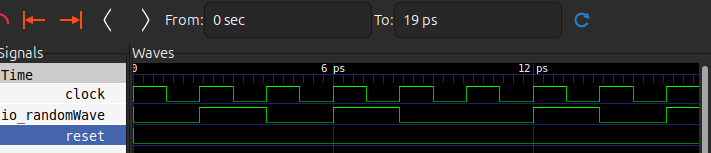
\includegraphics[width=\textwidth]{Images/verilator_waveformgenerator_screenshot.png} 
    \caption{Waveforms for generated SystemVerilog Verilator simulation}
    \label{fig:verilator_wave}
\end{figure}

Figure \ref{fig:verilator_wave} shows the waveform produced by simulating the clock generator using verilator. Section \ref{sub:verilator_test_driver} shows the process for generating the waveform shown in Figure \ref{fig:verilator_wave}. 


}%end chisel



\ifthenelse{\boolean{verilogversion} \and \boolean{chiselversion}}{   
%*********************************************************************************
\subsubsection{Comparison of Chisel and SystemVerilog Implementation of Waveforms}
%**********************************************************************************
In the Chisel implementation of the \texttt{waveFormGenerator}, the functionality is expressed using high-level abstractions. The \texttt{randomWave} is generated as a cyclic sequence of Boolean values, and its transitions are determined by a counter that increments on every clock cycle. Unlike the Verilog version, the Chisel implementation does not explicitly emulate timing delays but instead assumes uniform timing for each state in the sequence. 

While both implementations generate a \texttt{randomWave} and a clock-like signal, they differ in their timing behavior and functionality. The Verilog version explicitly specifies time delays for signal transitions and provides a clear stop condition using \texttt{\$stop}. The Chisel version is higher-level, more abstract, and assumes regular timing intervals without emulating the exact delays. This makes the Chisel version more suitable for hardware synthesis, where timing is managed by the clock, while the Verilog version offers precise control for simulation purposes.
}%end both true

%%%%%%%%%%%%%%%%%%%%%%%%%%%%%%%%%%%%%%%%%%%
\section{One-Input Combinational Circuits}
%%%%%%%%%%%%%%%%%%%%%%%%%%%%%%%%%%%%%%%%%%%
Combinational circuits are a fundamental type of digital circuit where the outputs are determined solely by the current inputs, without any memory or feedback elements. They perform logical and arithmetic operations based on Boolean algebra. Examples of combinational circuits include logic gates (AND, OR, NOT), arithmetic circuits (adders, subtractors), and data routing components (multiplexers, encoders). These circuits are deterministic, meaning their outputs are uniquely determined by the given inputs \cite{mano2017}.

%******************************
\subsection{Formal Description}
%******************************
A one-input combinational circuit is a digital logic circuit where the output depends solely on the value of a single binary input \( A \). Such circuits are governed by a Boolean function \( f(A) \), where \( f: \{0, 1\} \to \{0, 1\} \). The output is computed instantaneously based on the input value, with no memory or feedback elements involved. The behavior of the circuit can be described by a truth table, which enumerates the two possible input values (\( A = 0 \) and \( A = 1 \)) and their corresponding outputs (\( f(0) \) and \( f(1) \)). 

\begin{table}[H]
  \begin{center}
    \caption{One-input circuits.}
    \label{tab:one_input_circuits}
    \begin{tabular}{|c||c|c|c|}
      \hline
      A&  &  NOT&  BUFFER      \\ \hline \hline
      0&  &   1&       0    \\ \hline
      1&  &   0&       1    \\ \hline
    \end{tabular}
  \end{center}
\end{table}

\placedrawing[H]{figures/02_01_not.lp}{Graphic representation of the NOT and BUFFER circuits.}{fig:one_input_ckt}

Table \ref{tab:one_input_circuits} shows the truth table for a NOT gate, which inverts the input (\( f(A) = \neg A \)), and BUFFER (constant) circuit, which outputs a fixed value regardless of the input (\( f(A) = 0 \) or \( f(A) = 1 \)). Figure \ref{fig:one_input_ckt} shows the logic circuit symbol of the NOT and BUFFER combinational circuits. This is also called a gate symbol.

%***************************************************
\subsection{Physical Implementation of NOT Circuit}
%***************************************************
The physical implementation of a NOT circuit, or inverter, bridges the abstract concept of Boolean algebra with real-world digital hardware. A NOT gate takes a single input and produces an output that is its logical complement. In practice, this is typically achieved using transistor-based designs, such as CMOS (Complementary Metal-Oxide-Semiconductor) technology. 

The delay inherent in a NOT circuit, commonly referred to as the \emph{gate delay}, arises from the physical properties of the transistors and the interconnects. When the input changes state, the transistors must charge or discharge the capacitive load at the output. This charging and discharging process is influenced by factors such as the capacitance of the output node, the resistance of the transistors, and the speed of the power supply. As a result, the propagation delay, defined as the time taken for the output to reach a certain percentage of its final value after a change in input, becomes an important metric in digital circuit performance. 

Understanding where gate delays originate is important for designing circuits that meet timing requirements in high-speed applications. The interested reader can consult Appendix \ref{app:physical_implementations} for more information.

%%%%%%%%%%%%%%%%%%%%%%%%%%%
\section{Two-input gates}
%%%%%%%%%%%%%%%%%%%%%%%%%%%
Two-input gates depend on two binary inputs. Common two-input gates include AND, OR, XOR, NAND, and NOR. 

%*******************************
\subsection{Formal Description}
%******************************
Two-input gates are fundamental components in digital logic that perform Boolean operations on two binary variables, \( A \) and \( B \), to produce a single output \( f(A, B) \). Mathematically, these gates implement functions \( f: \{0, 1\} \times \{0, 1\} \to \{0, 1\} \), where the domain consists of all possible ordered pairs of binary inputs, and the range is restricted to binary outputs. 

Each type of two-input gate corresponds to a specific Boolean operation, such as AND (\( f(A, B) = A \land B \)). The behavior of these gates can be fully specified using truth tables, which enumerate all possible input combinations and their corresponding outputs.

\begin{table}[H]
  \begin{center}
    \caption{Two-input Combinational Gates Truth Table.}
    \label{tab:two_input_gates}
    \begin{tabular}{|c|c||c|c|c|c|c|c|}
      \hline
      $A$& $B$&   OR&        NOR&              AND&     NAND&              XOR&         XNOR \\ 
       &  &  $A\lor B$ & $\neg (A \lor B)$& $A\land B$& $\neg (A \land B)$&  $A\oplus B$&   $\neg (A \oplus B)$                              \\ \hline \hline
      0& 0&  0&         1&                 0&       1&                  0&           1\\ \hline
      0& 1&  1&         0&                 0&       1&                  1&           0\\ \hline
      1& 0&  1&         0&                 0&       1&                  1&           0\\ \hline
      1& 1&  1&         0&                 1&       0&                  0&           1\\ \hline
    \end{tabular}
  \end{center}
\end{table}

Table \ref{tab:two_input_gates} shows the truth table for combinational 2-input gates and Table \ref{tab:logic_gates_summary} shows the summary of their interpretations.

\begin{description}
\item[AND]: \( A \cdot B = AB \), where \( AB = 1 \) only if both \( A \) and \( B \) are 1, otherwise \( AB = 0 \). \\
    Numerical interpretation: Arithmetic product. \\
    Symbolic interpretation:  Gate, because \( A = 1 \) opens the way for \( B \). \\
    Alternative names: Conjunction, multiply gate, all-or-nothing gate \cite{boole1854book, rosen2018}.

\item[NAND]: \( \neg (A \cdot B) \), where the output is \( 0 \) only if both \( A \) and \( B \) are 1; otherwise, the output is \( 1 \). \\
    Symbolic interpretation: Universal gate. \\
    Alternative names: Sheffer stroke, negated AND gate \cite{sheffer1913, rosen2018}.

\item[OR]: \( A + B \), where \( A + B = 1 \) if at least one of \( A \) or \( B \) is \( 1 \); otherwise, \( A + B = 0 \). \\
    Symbolic interpretation: Inclusive OR. \\
    Alternative names: Disjunction, any-or-all gate \cite{rosen2018}.

\item[NOR]: \( \neg (A + B) \), where the output is \( 0 \) if at least one of \( A \) or \( B \) is \( 1 \); otherwise, the output is \( 1 \). \\
    Symbolic interpretation: Universal gate. \\
    Alternative names: Peirce arrow, negated OR gate \cite{peirce1885, rosen2018}.

\item[XOR]: Exclusive OR, because it excludes the case \( A = B = 1 \) in determining \( 1 \) on the output. \\
    \( A \oplus B = 1 \) when only one of the inputs \( A \) or \( B \) is \( 1 \). \\
    Logic interpretation: Conditioned inverter, i.e., \( \text{if } A = 0 \text{ then } A \oplus B = B, \text{ else } A \oplus B = B' \). \\
    Numerical interpretation: Modulo-2 sum. \\
    Symbolic interpretation: Anticoincidence. \\
    Alternative names: Either-or gate, modulo-2 adder \cite{shannon48, rosen2018}.

\item[XNOR]: \( \neg (A \oplus B) \). \\
    Symbolic interpretation: Coincidence. \\
    Alternative names: Equality gate, NOT XOR \cite{mano2017, rosen2018}.
\end{description}

\begin{table}[htbp]
\centering
\renewcommand{\arraystretch}{1.5} % Adjust row height
\setlength{\tabcolsep}{5pt} % Adjust column spacing
\begin{tabular}{|>{\centering\arraybackslash}p{2cm}|>{\centering\arraybackslash}p{3cm}|>{\centering\arraybackslash}p{2cm}|>{\centering\arraybackslash}p{5cm}|}
\hline
\textbf{Logic Gate} & \textbf{Numerical} & \textbf{Symbolic} & \textbf{Alternative Names} \\ \hline

OR  & Logical addition (no carry) \( A + B \) & \( A \lor B \) & Disjunction, Any-or-All Gate, Inclusive OR \\ \hline

NOR  & Complement of OR: \( 1 - (A + B) \) & \( \neg (A \lor B) \) & Peirce Arrow, Negated OR Gate, Universal Gate \\ \hline

AND & Logical multiplication \( A \cdot B \) & \( A \land B \) & Conjunction, Multiply Gate, All-or-Nothing Gate \\ \hline

NAND  & Complement of AND: \( 1 - (A \cdot B) \) & \( \neg (A \land B) \) & Sheffer Stroke, Negated AND Gate, Universal Gate \\ \hline

XOR  & Modulo-2 addition \( A \oplus B \) & \( A \oplus B \) & Exclusive OR, Modulo-2 Adder, Anticoincidence \\ \hline

XNOR  & Complement of XOR: \( 1 - (A \oplus B) \) & \( \neg (A \oplus B) \) & Exclusive NOR, Equality Gate, Coincidence \\ \hline

\end{tabular}
\caption{Summary of Logical Gates and their Interpretations}
\label{tab:logic_gates_summary}
\end{table}

Many of the historical names in \ref{tab:logic_gates_summary} stem from different disciplines. Terms like conjunction, disjunction, and negation originate from symbolic logic. Coincidence and anticoincidence were used in early telecommunications signal processing contexts. Practical descriptions like multiply gate and modulo-2 adder reflect the role of these gates in arithmetic and data processing. Modern digital logic has largely standardized the terms AND, OR, XOR, etc., as defined by IEEE and other standard bodies \cite{ieee_std_91}.

\placedrawing[H]{figures/02_07_two_input_gates.lp}{Graphical representation of the most used two-input gates.}{fig:graphical_gates}
Figure \ref{fig:graphical_gates} shows the graphical representations of logic gates. These originated from the need to visually depict logical operations in a way that facilitated the design and analysis of digital systems. These representations were inspired by symbolic logic and Boolean algebra, where logic functions were expressed using abstract symbols. Early pioneers, such as Claude Shannon, formalized the connection between Boolean algebra and electronic circuits, enabling the translation of logical expressions into circuit designs \cite{shannon48}. Over time, distinct shapes were assigned to each gate for clarity—such as the triangular symbol for NOT gates and the curved line for OR gates. Standardization efforts by organizations like the IEEE and IEC later codified these symbols, ensuring universal recognition and consistency in circuit diagrams \cite{ieee_std_91}. 


\placedrawing[H]{figures/02_08_non_inverting_gate_waveforms.lp}{Wave forms for the non-inverting gates.}{fig:waveforms}
Waveforms are tools used in digital logic for visualizing and analyzing the behavior of signals over time. They represent the changes in voltage levels for inputs, outputs, and intermediate nodes in a circuit, making it easier to understand timing relationships, transitions, and delays. The use of waveforms emerged alongside the development of oscilloscopes and other signal measurement tools in the early 20th century, as engineers needed a method to observe electrical signals in real-time. With the advent of digital systems, waveforms became a standard way to represent binary signals, where high and low voltage levels correspond to logical 1s and 0s, respectively. Waveforms allow engineers to verify the correct operation of logic circuits and diagnose timing-related issues such as glitches, race conditions, and setup/hold violations \cite{horowitz1993, ieee_waveform}. Their graphical nature complements schematic diagrams by providing temporal information that is not inherently visible in static circuit representations.


Figure \ref{fig:waveforms} shows the behavior of AND, OR and XOR gates. They are driven by the signals $A$ and $B$ represented in the first two wave forms. Besides the logic response to the inputs, timing characteristics are also shown. 
\begin{itemize}
    \item $t_+$: the positive transition time (the duration of the positive edge)
    \item $t_-$: the negative transition time (the duration of the negative edge)
    \item $t_{pLH}$: the propagation time  of the signal through the gate for the transition from Low to High
    \item $t_{pHL}$: the propagation time  of the signal through the gate for the transition from High to Low
\end{itemize}

We leave the treatment of timing to a course on digital logic design. It is a critical component in building working systems but is abstracted away in this book.

%%%%%%%%%%%%%%%%%%%%%%%%%%%
\section{Many-Input Gates}
%%%%%%%%%%%%%%%%%%%%%%%%%%%
Many-input gates are a generalization of 2-input gates, allowing the combination of more than two inputs into a single logical operation. For instance, an \( n \)-input AND gate outputs a logical \( 1 \) only when all \( n \) inputs are \( 1 \), while an \( n \)-input OR gate outputs \( 1 \) when at least one of the inputs is \( 1 \). As the number of inputs increases, the complexity of the gate's behavior grows exponentially, based on the number of possible input configurations.

Mathematically, the total number of distinct \( n \)-input gates is \( N^{2^n} \), where \( N \) represents the number of possible output values (typically \( N = 2 \) for binary logic), and \( 2^n \) is the total number of unique input configurations for \( n \) inputs. This exponential growth means that even for relatively small \( n \), the number of possible logic gates becomes vast and impractical to enumerate. For example, with \( n = 3 \), there are \( 2^{2^3} = 256 \) possible gates. For \( n > 2 \), Boolean algebra rules are necessary for simplifying and managing these functions, enabling the design of practical circuits without explicitly listing all possible gates.

In modern digital design, many-input gates are often implemented using a combination of smaller gates, as direct implementation can become physically and computationally impractical for large \( n \). For example, a 16-input AND gate might be constructed hierarchically by combining multiple 2-input AND gates. 

Let's consider some significant examples using verilog's ' (tick) symbol to denote negation:

\begin{itemize}
    \item (A')' = A
    \item AB + AB' = A(B + B') = A $\cdot$ 1 = A\\
    When B=1 the expression takes the value A, and when B=0 the expression still takes the value A, we conclude that the value of B does not matter and the expression takes the value A.
    \item A + A'B = A + B\\
    This can be proved by the truth table in Table \ref{tab:truth_table_proof}.
    \begin{table}[H]
  \begin{center}
    \caption{Truth table proof of A + A'B = A + B.}
    \label{tab:truth_table_proof}
    \begin{tabular}{|c|c||c|c|c||c|}
      \hline
      A& B&  A'& A'B& A+A'B& A+B   \\ \hline \hline
      0& 0&   1&   0&     0&   0   \\ \hline
      0& 1&   1&   1&     1&   1   \\ \hline
      1& 0&   0&   0&     1&   1   \\ \hline
      1& 1&   0&   0&     1&   1   \\ \hline
    \end{tabular}
  \end{center}
\end{table}
    \item A $\oplus$ B = (A' $\oplus$ B)' = (A $\oplus$ B')' = A' $\oplus$ B'
    \item A + B = (A'B')' \\
    From de Morgan's rule, A or B is 1 is equivalent to the fact that it is not true that A is 0 and B is 0.
    \item AB = (A' + B')'\\
    From de Morgan rule, A and B are 1 is equivalent to the fact that it is not true that A is 0 or B is 0.
\end{itemize}


%%%%%%%%%%%%%%%%%%%%%%%%%%%%%%%%%%%%%%%%%%%%%%%%%%%%%%%%%%%%%%%%%%%%%%%%%%%%%%%%%%%%%%%%%%%%%%%%%%%
\section{Generic combinational circuits}
%%%%%%%%%%%%%%%%%%%%%%%%%%%%%%%%%%%%%%%%%%%%%%%%%%%%%%%%%%%%%%%%%%%%%%%%%%%%%%%%%%%%%%%%%%%%%%%%%%%

\placedrawing[H]{figures/02_09_decoder.lp}{Decoder with $n$-bit input (DCDn).}{fig:decoder}

%*******************
\subsection{Decoder}
%********************
Figure \ref{fig:decoder} shows a generic $n$-bit decoder. A decoder is a combinational logic circuit that translates a binary-encoded input signal into a unique one-hot output. The term "one-hot" refers to a representation in which only one bit is set to '1', while all other bits are '0'. For example, in a 4-bit 1-hot code, valid outputs include 0001, 0010, 0100, and 1000. This encoding is commonly used in digital systems in control logic. It eliminates the need for decoding multiple bits simultaneously. 

\begin{figure}[h!]
\centering
\[
\begin{array}{|c|c||c|c|c|c|}
\hline
\text{Input} & \text{Input} & \text{Output} & \text{Output} & \text{Output} & \text{Output} \\
x_1 & x_0 &  y_3 &  y_2 & y_1 & y_0 \\
\hline
0 & 0 & 0 & 0 & 0 & 1 \\
0 & 1 & 0 & 0 & 1 & 0 \\
1 & 0 & 0 & 1 & 0 & 0 \\
1 & 1 & 1 & 0 & 0 & 0 \\
\hline
\end{array}
\]
\caption{Truth table for a 2-to-4 decoder. Each input combination activates one unique output in a one-hot encoding scheme.}
\label{fig:decoder_truth_table}
\end{figure}

A decoder takes an \(n\)-bit binary input and generates \(2^n\) output lines, with exactly one line active (logic high) for any given input combination. The structure of a decoder includes an array of logic gates that process the input bits and their complements to generate the appropriate output signals. For example, Figure \ref{fig:decoder_truth_table} shows the truth table for a 2-to-4 decoder. Figure \ref{fig:decoder_and_gates}a shows an elementary decode that output both $x_n$ and $\overline{x_n}$. Figure \ref{fig:decoder_and_gates}a shows the two input bits (\(x_1\) and \(x_0\)) and their negations (\(\overline{x_0}\) and \(\overline{x_1}\)) are used to drive four output signals (\(y_3, y_2, y_1, y_0\)). 

\placedrawing[H]{figures/02_10_recursive_decoder.lp}{Recursively defined 3-input decoder (DCD). {\bf a.} Elementary decoder (eDCD). {\bf b.} Two-input decoder (DCD2). {\bf c.} Three-input DCD (DCD3).}{fig:decoder_and_gates}

Decoders are widely used in digital systems for applications such as memory addressing, instruction decoding in processors, and enabling control signals in multiplexers. 


%#######################
% Decoder Code
%#######################
\ifthenelse{\boolean{verilogversion}}{
%*********************************************************
\subsubsection{Decoder (SystemVerilog)}
%*********************************************************    
\includeverilogcode[caption={Parameterized Decoder (SystemVerilog: dcdParameterized.sv)},     label={lst:verilog_decoder_parameterized}, firstline=8, firstnumber=8, lastline=999]{\verilogSourceDir/dcdParameterized.sv}

Listing \ref{lst:verilog_decoder_parameterized} shows a parameterized decoder implemented in SystemVerilog, which provides a scalable solution for decoding binary inputs to a one-hot encoded output. The design uses the shift operation to map the binary input to a specific bit position in the output. By using the parameter \texttt{INPUT\_WIDTH}, the module can dynamically adjust the size of the binary input and its corresponding one-hot output, with the output width automatically calculated as \(2^{\texttt{INPUT\_WIDTH}}\). This ensures that the decoder is flexible and reusable across various designs.

The key operation in the decoder is the left shift, expressed as \texttt{out = 1'b1 << in}, where the binary input \texttt{in} determines how many positions the single high bit is shifted. This eliminates the need for case statements or nested conditional logic. The shift operation is synthesis-friendly, allowing hardware tools to map the logic to a simple decoder circuit directly. 

\includeverilogcode[caption={4-to-16 Behavioral Decoder (SystemVerilog:dcd.sv)},     label={lst:verilog_decoder_4_to_16}, firstline=8, firstnumber=8, lastline=999]{\verilogSourceDir/dcd.sv}

Listing \ref{lst:verilog_decoder_4_to_16} shows a directly implemented 4-to-16 decoder.

}% End Verilog

\ifthenelse{\boolean{chiselversion}}{
%*************************************************
\subsubsection{Decoder (Chisel)}
%*************************************************
\includechiselcode[caption={Parameterized Decoder (Chisel: Decoder.scala)}, label={lst:chisel_decoder}, firstline=9, firstnumber=9, lastline=999]{\chiselSourceDir/Decoder.scala}

Listing \ref{lst:chisel_decoder} shows a Chisel parameterized decoder that can generate decoder logic based on a specified width. The decoder accepts a parameter, \texttt{n} the output width. This is also used to determine the number of input bits using the function \texttt{log2Ceil(n)}. This parameter dynamically adjusts the size of the output vector to \texttt{1 << inputWidth} (i.e., $2^{\text{inputWidth}}$), allowing the decoder to handle a variable number of input combinations. The use of a shift operation, \texttt{1.U << io.in}, implements the decoding logic by setting a single output bit corresponding to the binary input value.

\includechiselcode[caption={Instantiated 2-to-4 Decoder (Chisel: Decoder2to4.scala)}, label={lst:chisel_2to4_decoder}, firstline=8, firstnumber=8, lastline=999]{\chiselSourceDir/Decoder2to4.scala}

Listing \ref{lst:chisel_2to4_decoder} line 8 shows how simple it is to instantiate a decoder of any output width.

\includeverilogcode[caption={SystemVerilog Generated for Chisel firtool Decoder(4)}, label={lst:chisel_decoder_generated_verilog}, firstline=1, firstnumber=1, lastline=9999]{\verilogGeneratedByChiselSourceDir/Decoder2to4.v}

Chisel (or more precisely, firtool) automatically generates SystemVerilog for parameterized modules, while guaranteeing combinational logic. Listing \ref{lst:chisel_decoder_generated_verilog} shows the generated verilog code for a 2-to-4 decoder \texttt{Decoder(4)}.

\includeverilogcode[caption={Verilog Generated by sv2v for Decoder(4)}, label={lst:sv2v_decoder_generated_verilog}, firstline=1, firstnumber=1, lastline=9999]{\verilogGeneratedBySvtovSourceDir/Decoder2to4.v}

Commercial tools such as Vivado can directly elaborate and synthesize SystemVerilog. yosys, an open-source tool, can elaborate and synthesize some SystemVerilog statements but not all of them. We convert SystemVerilog to pure verilog using the open-source sv2v tool. Listing \ref{lst:sv2v_decoder_generated_verilog} line 11 shows that the shift semantics of the decoder are preserved in the generated verilog.

\includeverilogcode[caption={Verilog Elaborated by yosys for Decoder(4)}, label={lst:yosys_decoder_generated_verilog}, firstline=1, firstnumber=1, lastline=9999]{\verilogGeneratedByYosysSourceDir/Decoder2to4.v}

Listing \ref{lst:yosys_decoder_generated_verilog} shows the elaborated verilog produced by yosys. The shift operation has been transformed into logical operations. Lines 18 through 21 show the elaboration.

\begin{figure}[H]
    \centering
    
\includegraphics[width=0.8\textwidth]{\diagramsDir/Decoder2to4.png} 
    \caption{Generated Schematic of a yosys synthesized Chisel 2-to-4 Decoder.}
    \label{fig:ckt-2to4-decoder} % Use a label for cross-referencing
\end{figure}

After being elaborated by yosys, the schematic of \ref{fig:ckt-2to4-decoder} is automatically generated by netlistsvg.

}%End Chisel


\ifthenelse{\boolean{verilogversion} \and \boolean{chiselversion}}{   
%*********************************************************************************
\subsubsection{Decoder Language Comparison}
%**********************************************************************************

Chisel is a hardware construction language that generates hardware descriptions (e.g., Verilog) through the execution of Scala code. Its parameterized decoder uses functional programming paradigms to adjust the number of output bits based on the input width. The parameterized \texttt{Decoder} in Chisel is evaluated at \textbf{generation time}, which corresponds to the compile time of the Scala program, not the hardware synthesis. When the Chisel code is executed, the Scala runtime evaluates the parameterization and generates the corresponding Verilog/SystemVerilog code. This generated Verilog/SystemVerilog is then synthesized into hardware, meaning the parameterization is resolved before hardware runtime and does not exist dynamically in the final design.

Verilog lacks native parameterization and higher-level constructs, making it less flexible for scalable designs. A typical Verilog decoder implementation relies on manual enumeration or explicit assignment of output bits using case statements or combinational logic. 

SystemVerilog, as an enhancement of Verilog, introduces parameterization capabilities, which allow developers to create reusable and configurable hardware modules. A parameterized module in SystemVerilog uses \texttt{parameter} and \texttt{generate} constructs. Additionally, SystemVerilog supports advanced constructs like \texttt{logic} and \texttt{always\_comb}, which enforce combinational behavior. SystemVerilog parameterized designs are evaluated at \textbf{synthesis time}, when the hardware description is compiled and mapped into a physical implementation. These constructs allow for flexible and static parameterization, which the synthesis tool resolves before producing the final hardware netlist. 
}% End Both


%%%%%%%%%%%%%%%%%%%%%%%%
\subsection{Multiplexer}
%%%%%%%%%%%%%%%%%%%%%%%%%

A \textbf{multiplexer} (often abbreviated as \textit{mux}) is a combinational logic circuit that selects one of several input signals and forwards the selected input to a single output line. The input selection is controlled by a set of control signals or \textit{select lines}, which determine which input to pass to the output. A multiplexer with $n$ select lines can control $2^n$ inputs, making it a highly versatile and compact solution for signal routing in digital systems.

Multiplexers are widely used in digital design due to their ability to manage multiple signals within a system efficiently. In arithmetic circuits, multiplexers are often used for operations like selecting between different data sources or routing data to various processing units. They are also important components in larger systems such as CPUs, where they help implement control logic, ALU operation selection, and pipeline data forwarding. For example, in a microprocessor, a multiplexer might be used to select between input operands for an arithmetic operation based on the current instruction.

Multiplexers are used because they minimize the number of physical connections and wires required in a circuit. By reducing the need for separate connections for each input-output pair, a multiplexer allows for more efficient circuit designs. Additionally, they enhance the scalability of systems, because additional inputs can be accommodated by increasing the number of select lines. 

%**********************************
\subsection{Elementary Multiplexer}
%**********************************
\placedrawing[H]{figures/02_11_mux.lp}{Elementary multiplexer (eMUX). {\bf a.} The circuit structure: an eDCD serially connected with an AND-OR circuit. {\bf b.} The logic symbol.}{fig:mux}

Any combinational circuit can be expressed using only NAND functions. But a more interesting "fundamental brick" could be a circuit corresponding to the ubiquitous {\bf {\em if-then-ellse}} statement. It is the elementary multiplexer (eMUX) represented in Figure \ref{fig:mux}, and shows:

\begin{center} O = {\bf if} (S) {\bf then} I1 {\bf else} I0 \end{center}

%**********************************
\subsection{Many-input Multiplexer}
%**********************************

Figure \ref{fig:gen_mux} shows a many-input multiplexer. It takes bits from $m=2^n$ inputs selected by a $n$-bit code.

\placedrawing[H]{figures/02_12_mux_generalized.lp}{The general definition of the multiplexer circuit (MUXn). {\bf a.} The structure of MUXn: a DCDn serially connected with a $m=2^n$ ANDs on the first level of an AND-OR structure. {\bf b.} The logic symbol for MUXn.}{fig:gen_mux}

%#######################
% Multiplexer Code
%#######################
\ifthenelse{\boolean{verilogversion}}{
%*********************************************************
\subsubsection{Multiplexer (SystemVerilog)}
%*********************************************************    
\includeverilogcode[caption={16-to-1 single bit Multiplexer (SystemVerilog: mux.sv)},     label={lst:verilog_mux4}, firstline=8, firstnumber=8, lastline=999]{\verilogSourceDir/mux.sv}

Listing \ref{lst:verilog_mux4} implements a 16-to-1 single bit multiplexer. The module takes three inputs: a 16-bit vector \texttt{muxIn}, a 4-bit selector \texttt{muxSel}, and produces a single 1-bit output \texttt{muxOut}. The selector \texttt{muxSel} determines which bit of the 16-bit input vector is routed to the output. This is achieved through the indexing operation \texttt{muxIn[muxSel]}, which dynamically selects the bit of \texttt{muxIn} corresponding to the value of \texttt{muxSel}.

This design is both compact and efficient, leveraging Verilog's built-in array indexing capabilities. It allows the multiplexer to be easily scaled by adjusting the widths of \texttt{muxIn} and \texttt{muxSel}. Such multiplexers are fundamental building blocks in digital systems, often used to select between multiple data sources or routes in logic circuits, enabling dynamic and efficient data flow management.
}% End Verilog Code

\ifthenelse{\boolean{chiselversion}}{
%*************************************************
\subsubsection{Parameterized Bus Multiplexer (Chisel)}
%*************************************************
A \textit{bus} in digital systems is a collection of parallel lines or pathways used to transfer data between components within a system. Each line in a bus corresponds to a bit in the data, allowing the bus to carry multi-bit data simultaneously. Buses are parameterized by their width, which determines how many bits can be transmitted at once, and are used to connect various hardware components, such as processors, memory, and peripherals. For example, a 32-bit bus can carry 32 bits of data in parallel. 

\includechiselcode[caption={Parameterized Bus Type Multiplexer (Chisel: MultiplexerGenericType.scala)}, label={lst:chisel_muxT}, firstline=9, firstnumber=9, lastline=9]{\chiselSourceDir/MultiplexerGenericType.scala}


\addcontentsline{toc}{paragraph}{gen vs dataType - Chisel} \index{Chisel!gen} \index{Chisel!dataType}
Listing \ref{lst:chisel_muxT} shows a parameterized bus multiplexer in Chisel where the type of the bus is also parameterized using \texttt{[T <: Data](gen: T)]}. In Chisel, parameterizing modules with type parameters is a common practice to create reusable and modular designs. The choice between using \texttt{gen} and \texttt{dataType} depends on the context and the semantics of the module being designed. Each serves a slightly different purpose depending upon the intended hardware abstraction.

The \texttt{gen} parameter is well-suited when the type represents a \textit{blueprint} for generating multiple hardware elements. This is particularly relevant in cases where the module processes or instantiates multiple instances of the same type, such as multiplexers or reusable modules like FIFO queues and bus interfaces. For example, in Listing \ref{lst:chisel_muxT}, a multiplexer uses \texttt{gen} to define the type of data inputs and outputs, emphasizing that multiple identical instances are being handled within the hardware structure. 

 Given scala's generic types and type checking capabilities, it would be desirable to parameterize the bus type. Unfortunately, when generating hardware, this can sometimes appear as an invalid type conversion even if all interfaces are instantiated with \texttt{UInt<>}. Therefore, \textbf{ \textit{in this book, we have specified all classes to use \texttt{UInt}. This more closely aligns to verilog wires. }}Where possible, inside implementations, we still strive to ensure type safety using conversions such as \texttt{.asBool} and \texttt{.asSInt}, etc. 

\includechiselcode[caption={Parameterized Bus Width Multiplexer (Chisel: Multiplexer.scala)}, label={lst:chisel_mux}, firstline=9, firstnumber=9, lastline=20]{\chiselSourceDir/Multiplexer.scala}

Listing \ref{lst:chisel_mux} shows a bus multiplexer implemented as a class named \texttt{class Multiplexer}. This class is parameterized by the number of inputs (\texttt{n}) and the width of the bus (\texttt{width}). As shown on lines 14 through 16, all inputs and outputs are of type \texttt{UInt}  The class ensures through \texttt{require} statements that the number of inputs is both greater than zero and a power of two. 

The I/O bundle defines the interface for the multiplexer. It includes a vector (bus) of inputs, a selection signal, and the output. The size of the selection signal is calculated using \texttt{log2Ceil}, ensuring that it has enough bits to address all the inputs. The core logic of the multiplexer is implemented in a single line \texttt{io.output := io.inputs(io.select)}, where the output is assigned the value of the selected input. This is performed using Chisel’s vector indexing.

In Scala, a companion object is an object that shares the same name as a class and is defined in the same file. It acts as a singleton instance and provides a convenient way to group static-like methods and values associated with the class. Companion objects are particularly useful for factory methods, constants, or utility functions related to the class. Since they are in the same scope, companion objects and their corresponding classes can access each other's private members. This feature allows Scala developers to maintain clean and organized code, while still supporting the functional programming paradigm by avoiding the need for static members like in Java.

\includechiselcode[caption={Parameterized Bus Width Multiplexer Companion Object (Chisel: Multiplexer.scala)}, label={lst:chisel_mux_companion}, firstline=22, firstnumber=22, lastline=30]{\chiselSourceDir/Multiplexer.scala}

Listing \ref{lst:chisel_mux_companion} shows the companion object. The \texttt{Multiplexer} \textit{object} provides a factory method for creating and connecting instances of a parameterized multiplexer. The method takes a \texttt{Vec[UInt]} of inputs, and a \texttt{UInt} that specifies the selection signal for the multiplexer. After the module is instantiated, its I/O ports are connected. The \texttt{mux.io.inputs} port is connected to the \texttt{inputs} vector, and the \texttt{mux.io.select} port is connected to the \texttt{select} signal. Finally, the \texttt{apply} method returns the \texttt{mux.io.output}, providing the result of the multiplexer to the caller. 

\includechiselcode[caption={4-to-1 8-bit Bus Multiplexer (Chisel: Mux4.scala)}, label={lst:chisel_mux4}, firstline=8, firstnumber=8, lastline=999]{\chiselSourceDir/Mux4.scala}

Listing \ref{lst:chisel_mux4} shows an instantiation of a multiplexer with four 8-bit inputs. It uses the companion object to connect the signals. If the I/O signals retain the same names as the Multiplexer class, the 4-to-1 8-bit bus multiplexer could have been instantiated the same way as the 2-to-4 decoder shown in Listing \ref{lst:chisel_2to4_decoder} - \texttt{class Mux4 extends Multiplexer(4)}. However, it is often more convenient for users of hardware libraries to see the I/O definitions in the leaf class. Generally, we try to follow this design principle for instantiated Chisel hardware and so Listing \ref{lst:chisel_mux4} fully specifies the I/O signals.

\begin{figure}[H]
    \centering
    
\includegraphics[width=0.7\textwidth]{\diagramsDir/Mux4.png} 
    \caption{Generated Schematic of a yosys Elaborated Chisel 4-to-1 Multiplexer.}
    \label{fig:mux4} 
\end{figure}

Figure \ref{fig:mux4} shows the hierarchical schematic after yosys elaboration.

\begin{figure}[H]
    \centering
    
\includegraphics[scale=0.25]{\diagramsDir/Mux4_flat.png} 
    \caption{Generated Schematic of a yosys Elaborated and Flattened Chisel 4-to-1 Multiplexer.}
    \label{fig:mux4_flat} 
\end{figure}

Figure \ref{fig:mux4_flat} shows the schematic after the elaborated design is flattened. It is built from multiple 2-to-1 multiplexers.

}% End Chisel Code

%%%%%%%%%%%%%%%%%%%%%%%%%%%
\subsection{Demultiplexer}
%%%%%%%%%%%%%%%%%%%%%%%%%%%
A demultiplexer, often abbreviated as "demux," is a combinational circuit that takes a single input and channels it into one of several output lines based on the value of a selection signal. It is effectively the reverse operation of a multiplexer, consolidating multiple inputs into a single output. A demultiplexer is characterized by its ability to control the routing of the input data to the desired output line, ensuring that only one output is active at a time. The selection signal's binary value governs the active output selection.

Demultiplexers are useful in digital systems for tasks requiring data distribution. For instance, they are employed in scenarios where a single source of information needs to be directed to one of many destinations. In data routing applications, demultiplexers help in reducing the complexity of data paths and enable efficient communication between components. Moreover, they are integral to memory addressing systems, where they are used to select specific memory locations for reading or writing operations.

\placedrawing[H]{figures/02_13_demux.lp}{Demultiplexer as a DCD whose outputs are ANDed with the one bit signal to be distributed according to the $n$-bit input code. }{fig:demux}

Figure \ref{fig:demux} shows the demultiplexer transfers the input signal X to one of the $m=2^n$ outputs, $y_0, y_1, \ldots, y_{m-1}$, indicated by the $n$-bit selection input, $x_0, x_1, \ldots, x_{n-1}$. In Figure \ref{fig:demux} a demultiplexer is built using a decoder which open only one of the $m$ AND gate sending the $X$ input to the selected output.

For example: if $$\{x_{n-1} x_{n-2}, \ldots, x_1, x_0\} = 00 \ldots 011$$ then
$$\{y_{m-1} y_{m-2} \ldots y_0 y_1\} = 00 \ldots 0X000$$

%#######################
% DeMltiplexer Code
%#######################
\ifthenelse{\boolean{verilogversion}}{
%*********************************************************
\subsubsection{Demultiplexer (SystemVerilog)}
%*********************************************************    
\includeverilogcode[caption={1-to-16 bit Demultiplexer (SystemVerilog: dMux.sv)}, label={lst:verilog_demux16}, firstline=8, firstnumber=8, lastline=999]{\verilogSourceDir/dMux.sv}

Listing \ref{lst:verilog_demux16} shows SystemVerilog code that implements a simple demultiplexer module, named \texttt{dMux}. This demultiplexer takes a input signal \texttt{dMuxEnable} and routes one-bit of it to one of the 16 output lines, represented by the vector \texttt{dMuxOut}, based on the 4-bit selection signal \texttt{dMuxIn}. Instead of left-shifting the number 1 as in the decoder, the one-bit value $X$ is left-positioned. The operation is performed using a left-shift operation, where the input signal \texttt{dMuxEnable} is shifted by the value of \texttt{dMuxIn}, effectively enabling only one bit in the 16-bit output vector.

The \texttt{dMuxEnable} input acts as a control signal, ensuring that no outputs are active when it is low. 

}% End Verilog Code

\ifthenelse{\boolean{chiselversion}}{
%*************************************************
\subsubsection{Parameterized Demultiplexer (Chisel)}
%*************************************************
\includechiselcode[caption={Parameterized Bus Demultiplexer (Chisel: Demultiplexer.scala)}, label={lst:chisel_demuxT}, firstline=9, firstnumber=9, lastline=999]{\chiselSourceDir/Demultiplexer.scala}

Listing \ref{lst:chisel_demuxT} shows a parameterized demultiplexer (demux) that can handle an arbitrary number of outputs of type \texttt{Vec[UInt]}. The \texttt{Demultiplexer} class that extends Chisel's \texttt{Module} class to create a hardware module. The module includes a requirement that the number of outputs must be a power of two, enforced by the \texttt{require} statement. 

The \texttt{io} bundle defines the interface for the module, consisting of an input signal of type \texttt{UInt(width.W)}, a selection signal of width \(\log_2(\texttt{numOutputs})\), and a vector of \texttt{numOutputs} output signals. The implementation defaults all output signals to zero using \texttt{foreach}, ensuring that only the selected output is driven by the input signal. This is achieved by indexing the output vector with the \texttt{select} signal, which determines the active output line.

Simlar to the Multiplexer, a companion object provides a convenient factory method for instantiating the demultiplexer. The \texttt{apply} method creates an instance of the \texttt{Demultiplexer} class and connects the provided input and selection signals to the instance's IO ports. 

\includechiselcode[caption={1-to-16 64-bit Bus Demultiplexer (Chisel: DeMux16.scala)}, label={lst:chisel_demux16}, firstline=9, firstnumber=9, lastline=999]{\chiselSourceDir/DeMux16.scala}

Listing \ref{lst:chisel_demux16} shows a \texttt{DeMux16} class that defines a 1-to-16 demultiplexer that operates on 64-bit buses. This module is implemented as a subclass of \texttt{Module}, making it a Chisel hardware component. Its interface, specified by the \texttt{io} bundle, includes a 64-bit input bus (\texttt{io.input}), a 4-bit selection signal (\texttt{io.select}) to determine the active output, and a vector of 16 output buses (\texttt{io.outputs}), each 64 bits wide. The selection signal uses a 4-bit width because \(\log_2(16) = 4\), allowing indexing of the 16 outputs.

The \texttt{DeMux16} class instantiates a parameterized demultiplexer from the \texttt{Demultiplexer} companion object. The input and selection signals (\texttt{io.input} and \texttt{io.select}) are passed as arguments to the \texttt{Demultiplexer} factory method, which returns a vector of 16 outputs. These outputs are directly assigned to \texttt{io.outputs}, ensuring that only the selected output is driven by the input signal, while the others remain zero.

}% End Chisel

%*********************************
\subsection{Seven-Segment Display}
%*********************************
A 7-segment display is a common example of a combinational circuit that illustrates the concept of many-input logic gates. It consists of seven individual segments, labeled a through g, which can be illuminated to form numerical digits (0–9). The control logic for a 7-segment display is designed as a combinational circuit that takes a binary-coded decimal (BCD) input, typically 4 bits, and determines which segments should be activated to display the corresponding digit. Each segment is controlled by a Boolean expression derived from the binary input, effectively making the display a complex many-input gate. The circuit highlights how combinational logic can efficiently decode binary inputs into human-readable visual representations.

% FIXME: Get a 7-segment only drawing
\placedrawing[H]{figures/01_03_7seg_and_adder.lp}{The version of digital circuits. {\bf a.} Logic circuit: trans-coder for seven-segment display. {\bf b.} Numeric circuit: four-bit numbers adder.}{fig:7_segment_display}

Figure \ref{fig:7_segment_display} shows the transcoder for a 7-segment display. It receives four-bit coded decimal numbers, from 0 to 9, and convert them in 7-bit codes, a to g, indicating the segments to be activated, according to Table \ref{tab:sevenSeg}.

The logic expression for the output {\tt a} is:
\begin{center}
$a =   B'_3 \cdot B'_2 \cdot B'_1\cdot B'_0  + B'_3 \cdot B'_2 \cdot B_1\cdot B'_0  +
        B'_3 \cdot B'_2 \cdot B_1\cdot B_0  + B'_3 \cdot B_2 \cdot B'_1\cdot B_0  + $ \\
        $B'_3 \cdot B_2 \cdot B_1\cdot B'_0  + B'_3 \cdot B_2 \cdot B_1\cdot B_0  +
        B_3 \cdot B'_2 \cdot B'_1\cdot B'_0  + B_3 \cdot B'_2 \cdot B'_1\cdot B_0  $
\end{center}
or a simpler version by negatin the negated function:
$$a =  (a')' =  (B'_3 \cdot B'_2 \cdot B'_1\cdot B_0  + B'_3 \cdot B_2 \cdot B'_1\cdot B'_0)' = (B'_3 \cdot B'_1 \cdot (B_2 \oplus B_0))' = B_3 + B_1 + (B_2 \oplus B_0)'$$


\begin{table}[H]
  \begin{center}
    \caption{Seven-segment display truth table.}
    \label{tab:sevenSeg}
    \begin{tabular}{|c||c|c|c|c||c|c|c|c|c|c|c|}
      \hline
     & $B_3$ & $B_2$ & $B_1$ & $B_0$ & a & b & c & d & e & f & g \\ \hline \hline
     0& 0 & 0 & 0 & 0 & 1 & 1 & 1 & 1 & 1 & 1 &   \\ \hline % 0
     1& 0 & 0 & 0 & 1 &    & 1 & 1 &    &    &    &   \\ \hline % 1
     2& 0 & 0 & 1 & 0 & 1 & 1 &    & 1 & 1 &    & 1 \\ \hline % 2
     3& 0 & 0 & 1 & 1 & 1 & 1 & 1 & 1 &    &    & 1 \\ \hline % 3
     4& 0 & 1 & 0 & 0 &    & 1 & 1 &    &    & 1 & 1 \\ \hline % 4
     5& 0 & 1 & 0 & 1 & 1 &    & 1 & 1 &    & 1 & 1 \\ \hline % 5
     6& 0 & 1 & 1 & 0 & 1 &    & 1 & 1 & 1 & 1 & 1 \\ \hline % 6
     7& 0 & 1 & 1 & 1 & 1 & 1 & 1 &    &    &    &   \\ \hline % 7
     8& 1 & 0 & 0 & 0 & 1 & 1 & 1 & 1 & 1 & 1 & 1 \\ \hline % 8
     9& 1 & 0 & 0 & 1 & 1 & 1 & 1 & 1 &    & 1 & 1 \\ \hline % 9
    \end{tabular}
  \end{center}
\end{table}

%#######################
% 7 Segment Display Code
%#######################
\ifthenelse{\boolean{verilogversion}}{
%*********************************************************
\subsubsection{Seven Segment Display (SystemVerilog)}
%*********************************************************    
\includeverilogcode[caption={Seven Segment Display (SystemVerilog: SevenSegmentDisplay.sv)},     label={lst:verilog_sevensegmentdisplay}, firstline=7, firstnumber=7, lastline=999]{\verilogSourceDir/SevenSegmentDisplay.sv}

Listing \ref{lst:verilog_sevensegmentdisplay} shows SystemVerilog code that implements a seven-segment display decoder. The module, named \texttt{sevenSegmDys}, has a 4-bit binary input, \texttt{number}, and a 7-bit output, \texttt{seg}, which controls the state of the seven segments (labeled a through g) of the display. 

The \texttt{always\_comb} block defines a combinational block that describes the behavior of the output of the circuit as a combination based on the value of the input variables. The blocking assignment, {\tt =}, is used to assure the combinational behavior.

The \texttt{case} statement maps each possible input value (0 through 9) to a corresponding 7-bit output pattern that activates the appropriate segments to display the digit. For example, the binary input \texttt{4'b0000} (decimal 0) results in the output \texttt{7'b1111110}, which lights up all segments except \texttt{g}, forming the number 0 on the display.

The module includes a \texttt{default} case that sets all segments to off (\texttt{7'b0000000}) for invalid inputs outside the range 0–9. By mapping each input to a fixed segment configuration, this module can be integrated into larger digital systems that require visual representation of numeric values, such as timers, calculators, or embedded control systems.
}%End SystemVerilog

\ifthenelse{\boolean{chiselversion}}{
%*************************************************
\subsubsection{Seven Segment Display (Chisel)}
%*************************************************
\includechiselcode[caption={Seven Segment Display (Chisel: SevenSegmentDisplay.scala)},     label={lst:chisel_sevensegmentdisplay}, firstline=8, firstnumber=8, lastline=999]{\chiselSourceDir/SevenSegmentDisplay.scala}

Listing \ref{lst:chisel_sevensegmentdisplay} shows the \texttt{SevenSegmentDisplay} class is a Chisel module that decodes a 4-bit binary input (\texttt{binIn}) into a 7-bit output (\texttt{segOut}) representing the activation of segments on a seven-segment display. The input, \texttt{binIn}, can take values from 0 to 9, and the module determines which segments (labeled \texttt{a} through \texttt{g}) should be illuminated to form the corresponding numeric digit on the display.

The \texttt{suggestName} method in Chisel provides a mechanism to assign meaningful, user-defined names to intermediate signals or wires within a hardware design. By default, Chisel generates arbitrary names for these components, which can make debugging and analyzing generated hardware descriptions (e.g., Verilog or FIRRTL) challenging. Using \texttt{suggestName}, designers can explicitly label signals with descriptive names that convey their purpose or function within the design, making the generated hardware more readable and easier to trace.

The decoding logic is implemented using a series of \texttt{when} and \texttt{elsewhen} constructs. Each condition compares \texttt{binIn} with a specific value and assigns a 7-bit binary pattern to \texttt{segOut}. Each bit in the pattern corresponds to one of the seven segments, where a \texttt{1} turns the segment on, and a \texttt{0} turns it off. For example, when \texttt{binIn} is \texttt{0}, the output is \texttt{1111110}, which activates all segments except \texttt{g} to display the digit \texttt{0}. Similarly, for \texttt{binIn = 8}, all segments are activated (\texttt{1111111}). A default value of \texttt{0000000} is set for \texttt{segOut} to ensure all segments are off in case of invalid input.

In Chisel 6.6, the use of the \texttt{switch} function is discouraged because it often leads to less modular and harder-to-read code, especially in large designs. The \texttt{switch} function can introduce an implicit and tightly coupled relationship between the control signal and the cases, reducing flexibility and increasing the risk of errors during refactoring. Instead, Chisel promotes the use of more functional constructs like pattern matching or chained \texttt{when} statements which makes the design less prone to subtle bugs.

\includeverilogcode[caption={Propagation of suggestName() after yosys Elaboration (Generated SystemVerilog: yosys/SevenSegmentDisplay.v)},     label={lst:verilog_yosys_sevensegmentdisplay}, firstline=122, firstnumber=122, lastline=128]{\verilogGeneratedByYosysSourceDir/SevenSegmentDisplay.v}

The snippet in Listing \ref{lst:verilog_yosys_sevensegmentdisplay} shows that the signal names are propagated through to the synthesized design.

\begin{figure}[H]
    \centering
    
\includegraphics[scale=0.5]{\diagramsDir/SevenSegmentDisplay.png} 
    \caption{Generated Schematic of SevenSegmentDisplay Using \texttt{when} statements.}
    \label{fig:7seg_schematic} 
\end{figure}

Figure \ref{fig:7seg_schematic} shows the schematic after yosys elaboration. Unfortunately, netlistsvg does not retain the names even though they are in the generated verilog file.

%*********************************************************************************
\subsubsection{Seven Segment Display Using MuxSelect}
%**********************************************************************************
In Chisel, there are several constructs that can produce hardware in various forms. See Chapter \ref{chapt:perf_digital_logic} Section \ref{sec:muxcase} for details of using \texttt{when}, vs. \texttt{switch}, vs. \texttt{MuxCase}. From a programmer's point of view, \texttt{when} is likely the most familiar. However, \textbf{\textit{ \texttt{when} will priority encode complex signals.}} In the case of the Seven Segment Display, where all the conditions are independent, it will generate the signals in parallel.

\includechiselcode[caption={Seven Segment Display Using MuxCase (Chisel: SevenSegmentDisplayMuxCase.scala)},     label={lst:chisel_sevensegmentdisplay_muxcase}, firstline=43, firstnumber=43, lastline=54]{\chiselSourceDir/SevenSegmentDisplayMuxCase.scala}

When the designer wants \textbf{\textit{to guarantee parallel generation of hardware, \texttt{MuxCase} is preferred.}} Listing \ref{lst:chisel_sevensegmentdisplay_muxcase} shows the Chisel code using \texttt{MuxCase} instead of \texttt{when}.

\begin{figure}[H]
    \centering
    
\includegraphics[scale=0.25]{\diagramsDir/SevenSegmentDisplayMuxCase_not_asic.png} 
    \caption{Generated Schematic of SevenSegmentDisplay Using MuxCase.}
    \label{fig:7seg_schematic_muxcase} 
\end{figure}

Figure \ref{fig:7seg_schematic_muxcase} shows the schematic generated after yosys synthesis of the \texttt{MuxCase} Chisel code. Note that all multiplexers are reduced to parallel logic. However, it is also a lot of logic.

\begin{figure}[H]
    \centering
    
\includegraphics[scale=0.5]{\diagramsDir/SevenSegmentDisplayMuxCase_synth_flat.png} 
    \caption{Generated Schematic of SevenSegmentDisplay Using MuxCase and Skywater 130nm ASIC Technology files.}
    \label{fig:7seg_schematic_muxcase_asic} 
\end{figure}

Figure \ref{fig:7seg_schematic_muxcase_asic} shows the schematic generated after yosys synthesis of the \texttt{MuxCase} Chisel code with optimization guided by the Skywater CMOS 130nm technology library. Note that most of the gates are now NAND/NOR which are more efficient in CMOS implementations. 

\begin{figure}[H]
    \centering
    
\includegraphics[scale=0.5]{\diagramsDir/SevenSegmentDisplayMuxCase_synth.png} 
    \caption{Generated Schematic of SevenSegmentDisplay Using MuxCase Showing Exact Standard Cell Skywater 130nm ASIC Cells.}
    \label{fig:7seg_schematic_muxcase_asic_130} 
\end{figure}

Figure \ref{fig:7seg_schematic_muxcase_asic_130} shows the schematic generated after yosys synthesis of the \texttt{MuxCase} Chisel code with optimization guided by the Skywater CMOS 130nm technology library and the exact library cells selected from the Skywater library. The library has efficient implementations of 3-input gates. That selection is reflected in the synthesized design.

}%End Chisel



\ifthenelse{\boolean{verilogversion} \and \boolean{chiselversion}}{   
%*********************************************************************************
\subsubsection{Seven Segment Display Language Comparison}
%**********************************************************************************
The Chisel and SystemVerilog implementations both utilize conditional logic. Chisel uses \texttt{when} statements, while SystemVerilog uses a \texttt{case} statement within an \texttt{always\_comb} block. The primary decoding functions are both about the same number of lines of code. 

SystemVerilog's \texttt{always\_comb} guarantees that the logic produced is purely combinational, making the designer's intent explicit. In contrast, Chisel does not inherently enforce combinational logic; it depends on how constructs like \texttt{when} are used. For instance, \texttt{when} can describe sequential behavior if used with registers, but in the given example, the direct use of \texttt{:=} ensures combinational behavior.

}
%################################
% End Seven Segment Display Code
%################################


%%%%%%%%%%%%%%%%%%%%%%%%%%%%%%%%%%%%%%%%%%%%%%%%%
\section{Behavioral vs. Structural Descriptions}
%%%%%%%%%%%%%%%%%%%%%%%%%%%%%%%%%%%%%%%%%%%%%%%%%
Digital circuits can be described using two primary approaches: by defining their functional behavior or by specifying their internal structure. A behavioral description focuses on the circuit's input-output relationships, detailing what the circuit does without concern for how it is implemented internally. Conversely, a structural description specifies the arrangement and interconnection of the components that make up the circuit, providing a blueprint for how the desired functionality is achieved. 

The design of digital systems is inherently a \textbf{hierarchical process}. It begins with a top-level module that represents the overall system and is populated by submodules. Each submodule is defined similarly, with the process continuing until the simplest modules are reached. These basic modules are described directly, either through functional descriptions or by mapping to primitive hardware elements. This hierarchical organization allows for clear abstraction and separation of concerns, enabling designers to manage complexity effectively and focus on smaller, more manageable parts of the system.

One of the defining characteristics of digital design is \textbf{modularity}. In this approach, a complex problem is decomposed into smaller, simpler problems that are solved independently. This process is repeated recursively until the simplest possible components are identified and implemented. Modularity facilitates the reuse of identical modules throughout the design, enabling replication of the same component multiple times. This not only reduces development effort but also ensures consistency and reliability across the system. Furthermore, modular design supports scalability and maintainability, as individual modules can be optimized or replaced without affecting the rest of the system.

\placedrawing[h]{figures/01_04_4bit_adder.lp}{{\bf Hierarchical Decomposition Adder Modules.} {\small {\bf a.} Top-level 2-input 4-bit adder. {\bf b.} The structure of a 3-input 4-bit adder.} }{fig:hierarchical_adders}

Figure \ref{fig:hierarchical_adders}a shows an adder module. No indication of how this module is implemented is provided. We infer from its name that it adds two 4-bit numbers. Figure \ref{fig:hierarchical_adders}b shows a 3-input 4-bit adder composed of two 2-input 4-bit adders. While the module {\tt adder} is a {\em behavioral} description,
the module {\tt threeAdder} is a {\em structural} one. The first
tells us {\em what} is the function of the module, and the second
tells us {\em how} its functionality is performed by using a
structure containing two instantiation of a previously defined
subsystems, and an internal connection.




%%%%%%%%%%%%%%%%%%%%%%%%%%%%%%%%%%%%%%%%%%%%%%%%%%
\section{Adders}
%%%%%%%%%%%%%%%%%%%%%%%%%%%%%%%%%%%%%%%%%%%%%%%%%%
Adders are fundamental components in digital computing systems. At the core of processors, adders enable basic addition and form the building blocks for more complex arithmetic units, such as subtractors, multipliers, and dividers. An adder's efficiency directly impacts a processor's overall performance, as addition is one of the most frequently executed operations in computing.

%******************************
\subsection{Behavioral Adders}
%******************************
Behavioral adders describe what the circuit should do without specifying how it is implemented at the gate level. In contrast, specific adders, such as a carry-lookahead adder or a Kogge-Stone adder, describe the precise gate-level implementation of the addition operation. When synthesized using a tool like CIRCT, the \texttt{BehavioralAdder} would be converted into a hardware implementation that depends on the synthesis tool's optimization strategies. Typically, the synthesis tool would select an efficient adder architecture based on the target hardware platform and constraints. This could include ripple-carry, carry-lookahead, or other optimized implementations. The use of behavioral descriptions provides flexibility, as the specific implementation details are deferred to the synthesis process, enabling the designer to focus on functionality rather than low-level hardware details.

\ifthenelse{\boolean{chiselversion}}{
%*************************************************
\subsubsection{Parameterized Abstract Adder (Chisel)}
%*************************************************
\includechiselcode[caption={Parameterized Abstract Adder (Chisel: Adder.scala)}, label={lst:chisel_adder_abstract}, firstline=8, firstnumber=8, lastline=999]{\chiselSourceDir/adders/Adder.scala}

Listing \ref{lst:chisel_adder_abstract} shows code that defines an abstract class \texttt{Adder}, which provides a framework for creating parameterized adder modules in Chisel. The class requires a \texttt{width} parameter, which specifies the bit-width of the inputs and outputs. The \texttt{Adder} class requires a width greater than zero to ensure valid hardware design, and this is enforced by the \texttt{require} statement. The \texttt{io} interface is defined using a \texttt{Bundle} that encapsulates three signals: \texttt{a}, \texttt{b}, and \texttt{sum}. The \texttt{a} and \texttt{b} signals are inputs of type \texttt{UInt} with the specified \texttt{width}, representing the operands of the adder. The \texttt{sum} signal is an output of type \texttt{UInt} with the specified \texttt{width}, representing the computed sum of the inputs.

The class is marked as \texttt{abstract}, which means it cannot be instantiated directly. Instead, specific implementations of the adder, such as ripple-carry or carry-lookahead adders, can extend this base class to reuse the IO definitions and width constraints. Using an abstract base class like \texttt{Adder} provides several benefits. It ensures consistency in IO definitions, as all derived adder implementations inherit the same \texttt{io} interface, guaranteeing a uniform input-output structure across different adder designs. It promotes reusability by defining the \texttt{io} interface and width validation logic once in the base class, reducing code duplication and improving maintainability. The abstract base class introduces a level of abstraction by encapsulating common properties and behaviors, allowing derived classes to focus solely on implementing specific adder designs without redefining shared elements.

%************************************
\subsubsection{Precision in Addition}
%************************************
\begin{figure}[H]
    \centering
\[
\begin{array}{|c|c|c|c|c|c|c|}
\hline
\text{A (bin)} & \text{A (dec)} & \text{B (bin)} & \text{B (dec)} & \text{Sum (bin)} & \text{Sum (dec)} & \text{Overflow} \\
\hline
0000 & 0 & 0000 & 0 & 0000 & 0 & 0 \\
0001 & 1 & 0010 & 2 & 0011 & 3 & 0 \\
0111 & 7 & 0001 & 1 & 1000 & 8 & 0 \\
1111 & 15 & 0001 & 1 & 0000 & 0 & 1 \\
1010 & 10 & 0110 & 6 & 0000 & 0 & 1 \\
1110 & 14 & 1111 & 15 & 1101 & 13 & 1 \\
1111 & 15 & 1111 & 15 & 1110 & 14 & 1 \\
\hline
\end{array}
\]
    \caption{4-bit Behavioral Adder Partial Truth Table}
    \label{fig:4bit_adder_tt} 
\end{figure}

Figure \ref{fig:4bit_adder_tt} shows the partial truth table for a 4-bit behavioral adder. The column labeled overflow shows that $n$-bits in not sufficient to add two $n$-bit numbers. In general, adding two $n$-bit binary numbers requires $n+1$ bits to store the result.

Consider two $n$-bit binary numbers, $A$ and $B$, where each can be represented in the form:
\[
A = \sum_{i=0}^{n-1} a_i \cdot 2^i, \quad B = \sum_{i=0}^{n-1} b_i \cdot 2^i
\]

where $a_i, b_i \in \{0, 1\}$ are the binary digits (bits) of $A$ and $B$, respectively.

The range of each $n$-bit number can take any value from $0$ to $2^n - 1$. Therefore:
\[
0 \leq A \leq 2^n - 1, \quad 0 \leq B \leq 2^n - 1
\]

The maximum value of $A + B$ occurs when both $A$ and $B$ are at their maximum value, i.e., $A = 2^n - 1$ and $B = 2^n - 1$. In this case:
\[
A + B = (2^n - 1) + (2^n - 1) = 2^n + 2^n - 2 = 2^{n+1} - 2
\]

This shows that the result of $A + B$ can range from $0$ (minimum) to $2^{n+1} - 2$ (maximum). To store a result as large as $2^{n+1} - 2$, at least $n+1$ bits are required.

In the case of 4-bit unsigned numbers, observe that each operand, $A$ and $B$, can represent values from $0$ to $2^4 - 1 = 15$. When adding the two largest 4-bit numbers, $A = 15_{base10}$ and $B = 15_{base10}$, the result is $A + B = 30_{base10}$. To represent $30_{base10}$ in binary, at least 5 bits are required, as the binary representation is $11110_2$. 

\ifthenelse{\boolean{verilogversion}}{
%*************************************************
\subsubsection{2-input 4-bit Behavioral Adder (SystemVerilog)} 
%*************************************************

\includeverilogcode[caption={Behavorial 2-input 4-bit Adder (SystemVerilog: adder.sv)},     label={lst:verilog_adder}, firstline=9, firstnumber=9, lastline=999]{\verilogSourceDir/adder.sv}

Listing \ref{lst:verilog_adder} shows a 2-input 4-bit adder implemented in SystemVerilog. It is designed to perform 4-bit unsigned addition. It takes two 4-bit inputs, \texttt{in0} and \texttt{in1}, and produces a 4-bit output, \texttt{out}, representing the sum of the two inputs. The addition operation is performed using the \texttt{assign} statement, which continuously evaluates the sum of \texttt{in0} and \texttt{in1} and assigns the result to \texttt{out}.

This module does not include provisions for detecting overflow, which occurs when the result of the addition exceeds the 4-bit range (0 to 15). In such cases, the sum wraps around, effectively discarding the carry bit that exceeds the 4-bit width making it a modulo 16 adder. 
}%End verilog code


%*************************************************
\subsubsection{Parameterized Behavioral Adder (Chisel)} \label{sec:behavioral_addition}
%*************************************************
\includechiselcode[caption={Parameterized Behavioral Adder (Chisel)}, label={lst:chisel_adder_behavioral}, firstline=8, firstnumber=8, lastline=17]{\chiselSourceDir/adders/BehavioralAdder.scala}

Listing \ref{lst:chisel_adder_behavioral} shows code that defines a class \texttt{BehavioralAdder}, which extends the abstract \texttt{Adder} class to implement a simple, behavioral adder in Chisel. All interface IO are of type UInt. The class is parameterized by the width of the adder \texttt{width}. The addition operation is specified behaviorally using the expression \texttt{io.a + io.b}, which computes the sum of the two input signals and assigns it to the output signal \texttt{io.sum}. 

\textbf{An important point} is that Chisel will expand the result to keep full precision. In simulation, this may be the desired behavior. However, hardware cannot dynamically expand wires. Chisel leaves this decision to the programmer but synthesis requires fixed widths. Our behavioral adder implementation truncates the sum result to the width of the output wires using \texttt{(width -1, 0)} on line 16.

%***********************************
\subsection{4-bit Behavioral Adder}
%***********************************
\includechiselcode[caption={4-bit Behavioral Adder (Chisel: BehavioralAdder4.scala)}, label={lst:chisel_adder_behavioral4}, firstline=8, firstnumber=8, lastline=17]{\chiselSourceDir/adders/BehavioralAdder4.scala}

Listing \ref{lst:chisel_adder_behavioral4} shows a 4-bit behavioral adder that instantiates the class \texttt{BehavioralAdder}. 

\begin{figure}[H]
    \centering
    
\includegraphics[scale=0.95]{\diagramsDir/BehavioralAdder4.png} 
    \caption{High-level Schematic of a Behavioral 4-bit Adder.}
    \label{fig:4bit_adder_behavioral} 
\end{figure}

After yosys elaboration, both a high-level and flatted circuit diagram can be generated. Figure \ref{fig:4bit_adder_behavioral} shows the schematic for a high-level schematic. Figure \ref{fig:4bit_adder_synth} shows the schematic for a yosys synthesized and flattened 4-bit adder.

\begin{figure}[H]
    \centering
    
\includegraphics[scale=0.4]{\diagramsDir/BehavioralAdder4_flat.png} 
    \caption{Yosys Synthesized and Flattend Schematic of a Behavioral 4-bit Adder.}
    \label{fig:4bit_adder_synth} 
\end{figure}

}% End Chisel


%*****************************
\subsection{Structural Adders}
%*****************************

Computers use structural adders to perform arithmetic operations efficiently at the hardware level. A structural adder is a circuit composed of interconnected logic gates designed to compute the sum of binary numbers. These adders allow computations to occur in a predictable, deterministic manner, with a fixed propagation delay determined by the design. Unlike behavioral implementations, structural adders operate at the level of individual bits, ensuring that addition is performed in accordance with the system's clock cycle.

The concept of carry bits is central to structural adders. In binary arithmetic, when the sum of two bits exceeds the value that a single bit can represent, the excess is propagated as a carry bit to the next more significant bit. This mechanism ensures accuracy in multi-bit addition, but it also introduces challenges, such as carry propagation delays. 

In this Section, we only provide an overview of the simplest structural adders. Practical implementations with higher performance (and complexity) are covered in Chapter \ref{chapt:perf_digital_logic}.

%**********************
\subsubsection{Half Adder}
%**********************
\placedrawing[H]{figures/02_14_half_adder.lp}{Half adder (HA).The XOR circuit compute the {\em modulo-2} sum while the AND gate compute the carry value.}{fig:half_adder}

Figure \ref{fig:half_adder} shows the simplest adder - the \textit{half adder}. It adds two binary digits and produces a sum and a carry bit. To build a half adder we use an XOR circuit. The XOR circuit calculates the sum modulo 2 but does not differentiate between 0+0 and 1+1. This differentiation involves the calculation of the arithmetical overshoot, which we denote by carry (to the next binary order). The Carry signal is activated when both inputs are 1. Therefore, in addition to the XOR gate we must add an AND gate. The resulting circuit is called a \textit{half adder} because it does not take into account the carry signal provided by the previous binary order.

%**********************
\subsubsection{Increment}
%**********************
\placedrawing[H]{figures/02_15_increment.lp}{Increment circuit for 4-bit numbers (INC4) implemented by serially connected $4$ HAs.}{fig:incrementer}

Figure \ref{fig:incrementer} shows the schematic for a 4-bit incrementer that uses only half adders. Incrementing means adding 1 to a number. If {\tt inc = 1} the output $out_0 <= in'_0$  and {\tt cr} of $HA_0$ if it is activated command the increment for $HA_1$, and so on.

If each 2-input AND from $HA_i$ has, for example,  a propagation time, $t_{pAND2} = 1ns = 10^{-9}sec$, and the 2-input XOR has the propagation time, $t_{pXOR2} = 1.5ns$, then the total execution time for the INC4 circuit is:
$$t_{pINC4} = 3 \times t_{pAND2} + t_{pXOR2} = 4.5ns$$
Thus, the size of the $n$-bit number increment circuit, $S_{INCn}$, is proportional with the input size. However, the execution time, i.e., depth, $D_{INCn}$, is in the same order of magnitude:
$$S_{INCn} \in O(n)$$
$$D_{INCn} \in O(n)$$

The depth of the circuit can be reduced by increasing the size (but in the limits of the same magnitude order) using a prefix network such as a Kogge-Stone adder \cite{kogge1973parallel}. See Section \ref{sec:kogge-stone-adder}.

%******************************
\subsubsection{Full Adder (FA)}
%******************************
Half adders cannot handle carry inputs, leading to the development of the \textit{full adder}, which incorporates a carry input along with two operand inputs. The Full Adder (FA) adds two one-bit numbers with the carry provided from the previous binary position. It generates the sum and the carry value for the next binary position. In Figure \ref{fig:full_adder}a, a FA is composed of two HAs and an OR circuit used to propagate the carry generated by the first HA or by the second HA. The first FA adds the two input bits, A and B, while the second FA adds the value of the carry, C, generated by the previous binary order.

\placedrawing[H]{figures/02_16_adder_full.lp}{Adder. {\bf a.} Full Adder (FA). {\bf b.} 4-bit adder (ADD4).}{fig:full_adder}

%*******************************
\subsubsection{Ripple-Carry Adder} \label{sec:ripple-carry-adder}
%******************************
Figure \ref{fig:full_adder}b shows a schematic for a \textit{ripple carry adder} (RCA). Ripple-carry adders are one of the simplest and most fundamental types of binary adders. They work by connecting a series of full adders, each responsible for processing a single bit of the operands. The carry-out from each adder is propagated to the carry-in of the next, creating a "ripple" effect that moves from the least significant bit (LSB) to the most significant bit (MSB). 

While the design of ripple-carry adders is straightforward and easy to implement in hardware, their performance is limited by the sequential nature of carry propagation. The execution time, i.e., the maximum time interval from when an input changes until all the outputs of the circuit reach the correct final value, can be long. This time interval is due to propagation through logic gates on the longest path. In this case, the longest path is the one from input $C$ to output $C_{out}$. On this path there are 8 logic gates, one AND and one OR for each binary order. The delay for an addition operation increases linearly with the number of bits, as each bit must wait for the carry result from the preceding bit to be resolved. In the general case, the time is proportional to $n$ (it is in $O(n)$). 

%%%%%%%%%%%%%%%%%%%%%%%%%%%%%%%%%%%%%%%%%%%%%%%%%%
\section{Multipliers}
%%%%%%%%%%%%%%%%%%%%%%%%%%%%%%%%%%%%%%%%%%%%%%%%%%

%******************************
\subsection{Behavioral Multiplier}
%******************************
Similar to behavioral adders, behavioral multipliers describe what the circuit should do without specifying how it is implemented at the gate level. 

\ifthenelse{\boolean{chiselversion}}{
%*************************************************
\subsubsection{Parameterized Abstract Multiplier (Chisel)}
%*************************************************
\includechiselcode[caption={Parameterized Abstract Multiplier (Chisel: Multiplier.scala)}, label={lst:chisel_mult_abstract}, firstline=8, firstnumber=8, lastline=999]{\chiselSourceDir/multipliers/Multiplier.scala}

Listing \ref{lst:chisel_mult_abstract} shows an abstract multiplier. The \texttt{Multiplier} class is an abstract module in Chisel, designed to serve as a base for implementing various multiplier designs. The module defines the basic input-output (I/O) interface and enforces the requirement that the bit-width of the operands, specified by the \texttt{width} parameter, must be greater than zero. This ensures that any concrete multiplier inheriting from this class adheres to a consistent interface and valid configuration.

The I/O interface comprises two unsigned integer inputs, \texttt{a} and \texttt{b}, both of the specified \texttt{width}, a control input \texttt{isSigned}, and a single output, \texttt{result}, which provides the full precision product of the multiplication. The \texttt{isSigned} input determines whether the multiplication is interpreted as signed or unsigned, allowing the module to handle both arithmetic modes dynamically. The \texttt{result} output has a width of \texttt{2 * width}, reflecting the theoretical maximum number of bits required to store the result of multiplying two \texttt{width}-bit numbers, regardless of whether the operation is signed or unsigned. 


%*************************************************
\subsubsection{Parameterized Behavioral Multiplier (Chisel)}
%*************************************************
\includechiselcode[caption={Parameterized Behavioral Multiplier (Chisel: BehavioralMultiplier.scala)}, label={lst:chisel_mult_behavioral}, firstline=8, firstnumber=8, lastline=14]{\chiselSourceDir/multipliers/BehavioralMultiplier.scala}

Listing \ref{lst:chisel_mult_behavioral} shows a behavioral multiplier. The \texttt{BehavioralMultiplier} class is a concrete implementation of the abstract \texttt{Multiplier} class designed to perform both signed and unsigned multiplications dynamically, based on the \texttt{isSigned} input signal. This parameterized module accepts operands \texttt{a} and \texttt{b} of a specified bit \texttt{width}, with the result of the multiplication output on the \texttt{result} port. The \texttt{isSigned} input determines whether the multiplication is interpreted as signed or unsigned. When \texttt{isSigned} is asserted (equal to \texttt{1.U}), the operands are cast to signed integers (\texttt{SInt}) for multiplication, and the resulting signed product is cast back to an unsigned integer (\texttt{UInt}) for output. Conversely, if \texttt{isSigned} is deasserted (equal to \texttt{0.U}), the operands are treated as unsigned integers for multiplication.

The output \texttt{result} has a width of \texttt{2 * width}, ensuring sufficient precision to accommodate the maximum possible product of two \texttt{width}-bit numbers, whether signed or unsigned. 

}% End Chisel code

%******************************************
\subsection{Precision in Multiplication}
%*******************************************

\begin{figure}[H]
    \centering
\[
\begin{array}{|c|c|c|c|c|c|}
\hline
\text{A (bin)} & \text{A (dec)} & \text{B (bin)} & \text{B (dec)} & \text{Product (bin)} & \text{Product (dec)} \\
\hline
0001 & 1 & 0001 & 1 & 00000001 & 1 \\
0011 & 3 & 0010 & 2 & 00000110 & 6 \\
0111 & 7 & 0101 & 5 & 00101111 & 35 \\
1111 & 15 & 1111 & 15 & 11100001 & 225 \\
1000 & 8 & 1001 & 9 & 10010000 & 144 \\
1111 & 15 & 0001 & 1 & 00001111 & 15 \\
0110 & 6 & 0011 & 3 & 00010010 & 18 \\
\hline
\end{array}
\]
    \caption{4-bit Behavioral Multiplier Partial Truth Table for Unsigned Numbers}
    \label{fig:4bit_multiplier_tt_unsigned}
\end{figure}

Figure \ref{fig:4bit_multiplier_tt_unsigned} shows the partial truth table for a 4-bit behavioral multiplier using unsigned numbers. The results demonstrate that multiplying two $n$-bit numbers may require up to $2n$ bits to represent the full product.

Consider two $n$-bit binary numbers, $A$ and $B$, where each can be represented in the form:
\[
A = \sum_{i=0}^{n-1} a_i \cdot 2^i, \quad B = \sum_{i=0}^{n-1} b_i \cdot 2^i
\]

where $a_i, b_i \in \{0, 1\}$ are the binary digits (bits) of $A$ and $B$, respectively.

The maximum product occurs when both $A$ and $B$ are at their maximum value, i.e., $A = 2^n - 1$ and $B = 2^n - 1$. In this case:
\[
A \times B = (2^n - 1) \times (2^n - 1) = 2^{2n} - 2^n - 2^n + 1 = 2^{2n} - 2^{n+1} + 1
\]

This shows that the result of $A \times B$ can range from $0$ (minimum) to approximately $2^{2n}$ (maximum). To store a result as large as $2^{2n} - 1$, $2n$ bits are required.

In the case of 4-bit unsigned numbers, each operand, $A$ and $B$, can represent values from $0$ to $2^4 - 1 = 15$. When multiplying the two largest 4-bit numbers, $A = 15_{base10}$ and $B = 15_{base10}$, the result is $A \times B = 225_{base10}$. To represent $225_{base10}$ in binary, at least 8 bits are required, as the binary representation is $11100001_2$.

\begin{figure}[H]
    \centering
\[
\begin{array}{|c|c|c|c|c|c|}
\hline
\text{A (bin)} & \text{A (dec)} & \text{B (bin)} & \text{B (dec)} & \text{Product (bin)} & \text{Product (dec)} \\
\hline
0111 & 7 & 0101 & 5 & 00101111 & 35 \\
1001 & -7 & 0011 & 3 & 11011101 & -21 \\
0110 & 6 & 1100 & -4 & 11101100 & -24 \\
1010 & -6 & 1010 & -6 & 00110000 & 36 \\
1111 & -1 & 1111 & -1 & 00000001 & 1 \\
1000 & -8 & 0001 & 1 & 11111000 & -8 \\
0111 & 7 & 1111 & -1 & 11111001 & -7 \\
\hline
\end{array}
\]
    \caption{4-bit Behavioral Multiplier Partial Truth Table for Signed Numbers}
    \label{fig:4bit_multiplier_tt_signed}
\end{figure}

Figure \ref{fig:4bit_multiplier_tt_signed} shows the partial truth table for signed numbers. Here, the results indicate that $2n$ bits are also required to store the signed product. 

For signed numbers, represented using two's complement, the analysis differs slightly due to the sign extension for negative operands. In two's complement, the most significant bit (MSB) represents the sign, with $0$ for positive and $1$ for negative numbers. The value of an $n$-bit signed number $A$ is given by:
\[
A = -a_{n-1} \cdot 2^{n-1} + \sum_{i=0}^{n-2} a_i \cdot 2^i
\]

Similarly, for $B$:
\[
B = -b_{n-1} \cdot 2^{n-1} + \sum_{i=0}^{n-2} b_i \cdot 2^i
\]

The maximum and minimum values of $A$ and $B$ are $2^{n-1} - 1$ (maximum positive) and $-2^{n-1}$ (minimum negative), respectively. The maximum magnitude of the product occurs when one operand is at its maximum positive value and the other is at its minimum negative value:
\[
\text{Max Magnitude: } |A \times B| = (2^{n-1} - 1) \cdot 2^{n-1} = 2^{2n-1} - 2^{n-1}
\]

In this case, the signed product can range from:
\[
-2^{2n-2} \leq A \times B \leq 2^{2n-2} - 1
\]

Thus, $2n$ bits are still required to store the full result of signed multiplication to account for both the sign and the magnitude.

%**************************************************************************
\subsection{Two's Complement Multiplication and Intermediate Overflows}
%**************************************************************************

In two's complement multiplication, intermediate overflows that occur during the computation process generally do not affect the correctness of the final result, provided that the final result fits within the target bit range. This behavior arises due to the nature of two's complement arithmetic, which wraps values and preserves correctness when results are truncated to the appropriate bit width.

During multiplication in hardware implementations, intermediate results may produce higher-order bits that "overflow" beyond the required range. For example, multiplying two 4-bit numbers in two's complement may generate intermediate results that temporarily require more than 4 bits. These overflows occur due to the nature of the multiplication operation but are irrelevant to the correctness of the final result, provided the final result fits in 4 bits.

For a signed \(n\)-bit number in two's complement, the range of representable values is \(-2^{n-1}\) to \(2^{n-1} - 1\). As long as the final product lies within this range, any intermediate overflows are inconsequential. For example, multiplying \(-7\) (\(1001\)) and \(3\) (\(0011\)) in 4-bit two's complement results in \(11101101\) in 8 bits. When truncated back to 4 bits, the result is \(1101\), which correctly represents \(-21\).

Consider multiplying \(4\) (\(0100\)) and \(2\) (\(0010\)) and \(-1\) \(1111\) in 4-bit two's complement arithmetic:
\[
4 \times 2 = 8
\]
\[
0100 \times 0010 = 0000\_1000 = 1000
\]
8 is not representable in 2's complement 4-bits but ignoring the overflow and multiplying by $-1$ gives
\[
1000 \times 1111 = 0111\_1000 = 1000
\]

When truncated to 4 bits, the result becomes:
\[
1000
\]
This correctly represents \(-8\) in 4-bit two's complement arithmetic, demonstrating that intermediate overflows do not affect the correctness of the final result.

%**************************************************************************
\subsection{Handling Extended Results}
%**************************************************************************

In arithmetic and logical operations, the handling of the extended result, which refers to the extra bits generated during operations such as multiplication or addition, depends on the operation context, the target application, and the architecture. For example, multiplication of two \texttt{n}-bit numbers produces a \texttt{2n}-bit result. In many cases, the result is stored in its entirety, especially in applications that require high precision, such as digital signal processing (DSP) or scientific computing. Architectures like x86 provide instructions that store the low and high halves of the result in separate registers, enabling seamless access to the full \texttt{2n}-bit result.

Modern instruction set architectures (ISAs) often provide distinct opcodes for accessing either the low or high parts of the extended result. For example, in RISC-V, instructions like \texttt{MUL} produce the lower bits of a multiplication result, while \texttt{MULH} and \texttt{MULHU} are used to extract the higher bits for signed and unsigned operations, respectively. Alternatively, some architectures provide combined instructions that store the full-width result across multiple registers. The choice between retaining or discarding the extended result ultimately depends on application requirements, hardware resource constraints, and the overall design philosophy of the ISA. In many ALU designs, retaining the low bits is the default behavior, with access to the high bits provided through additional instructions or status flags for more specialized use cases.

%****************************************
\section{Multi-Function Arithmetic Units}
%****************************************

A multifunction arithmetic unit performs a variety of arithmetic operations such as addition, subtraction, and sometimes multiplication or division, on the same hardware unit. These units are typically designed to handle both signed and unsigned numbers and often support different operand sizes, such as 8-bit, 16-bit, 32-bit, or 64-bit operations. By sharing hardware resources among multiple operations, multifunction arithmetic units reduce the overall complexity of the system.

A multifunction arithmetic unit includes configurable control signals, sometimes called an operation code or opcode, that dictate the operation to be performed. For example, an opcode may specify whether the operation is addition or subtraction, whether the operands are signed or unsigned, and the size of the operands. 

 Adding a sign/unsigned control bit to an arithmetic unit is a simple example of a multifunction arithmetic unity that enable the same hardware to handle both signed and unsigned operations. In the context of binary arithmetic, signed and unsigned numbers differ primarily in their interpretation of the most significant bit (MSB). For unsigned numbers, the MSB contributes solely to the magnitude of the value, while for signed numbers in two's complement representation, the MSB serves a dual purpose: it indicates the sign of the number (0 for positive, 1 for negative) and also contributes to its magnitude in determining the overall value. 
 
 Adding a control signal for selecting between addition and subtraction further enhances the functionality of the unit. Subtraction can be implemented using the same hardware as addition by negating one of the operands, which involves flipping the bits and adding one. With two control signals—one for signed/unsigned selection and another for addition/subtraction—the unit becomes a multifunction adder/subtractor, capable of performing basic arithmetic operations across a wide range of use cases.

When additional operations such as bitwise logical operations (AND, OR, XOR) and shifting (logical, arithmetic, and rotate) are incorporated into the same hardware unity, this is typically called an arithmetic logic unit (ALU). The control signals that specify a particular operation are referred to as an opcode. An ALU is the computational heart of a processor.

%************************
\subsection{Subtraction}
%************************
%*************************************
\subsubsection{Behavioral Adder/Subtractor}
%**************************************
Similar to behavioral addition described in Section \ref{sec:behavioral_addition}, we can also provide for behavioral subtraction. A subtractor can share hardware with an adder making an adder/subtractor the simplest multifunction arithmetic unit.

\ifthenelse{\boolean{chiselversion}}{

\includechiselcode[caption={Behavioral Adder/Subtractor (Chisel: BehavioralAdderSubtractor.scala)}, label={lst:chisel_addersubtractor_behavioral}, firstline=8, firstnumber=8, lastline=22]{\chiselSourceDir/addersubtractors/BehavioralAdderSubtractor.scala}

Listing \ref{lst:chisel_addersubtractor_behavioral} shows a behavioral adder/subtractor. 
The \texttt{BehavioralAdderSubtractor} class defines a parameterized hardware module in Chisel for performing addition or subtraction of unsigned integers. The module is parameterized by a \texttt{width}, allowing it to handle operands of varying bit widths. The input-output interface (\texttt{io}) is defined as a \texttt{Bundle} that includes two inputs (\texttt{a} and \texttt{b}), each of type \texttt{UInt} with the specified bit width, a control signal (\texttt{subtract}) to select the operation, and an output (\texttt{result}) that provides the computed value.

The core computation is performed using a \texttt{Mux} construct, which selects between addition (\texttt{io.a + io.b}) and subtraction (\texttt{io.a - io.b}) based on the value of the \texttt{subtract} signal. If \texttt{subtract} is 0, addition is performed; otherwise, subtraction is performed. 

The result of the operation is assigned to the \texttt{io.result} output. To ensure that the output adheres to the specified bit width, the \texttt{fullResult} is truncated using \texttt{(width - 1, 0)}, which extracts only the least significant \texttt{width} bits of the result. This ensures that the output does not exceed the desired width, even in cases of overflow or underflow. 

\includechiselcode[caption={4-bit Behavioral Adder/Subtractor (Chisel: BehavioralAdderSubtractor4.scala)}, label={lst:chisel_addersubtractor_behavioral4}, firstline=17, firstnumber=17, lastline=17]{\chiselSourceDir/addersubtractors/BehavioralAdderSubtractor4.scala}

Listing \ref{lst:chisel_addersubtractor_behavioral4} shows an instantiation of a Chisel 4-bit behavioral adder/subtractor. The \texttt{BehavioralAdderSubtractor4} module defines an input-output interface (\texttt{io}) consisting of two 4-bit unsigned inputs (\texttt{a} and \texttt{b}), a 1-bit control signal (\texttt{subtract}), and a 4-bit unsigned output (\texttt{sum}). 

The arithmetic operation itself is delegated to a reusable module called \texttt{BehavioralAdderSubtractor}, which is invoked with the necessary parameters, including the two input values (\texttt{a} and \texttt{b}), the \texttt{subtract} control signal, and the bit width of the operation (4 bits in this case). The result of the operation is assigned to the \texttt{sum} output. 

}%End Chisel Code

%*************************************
\subsubsection{Structural Subtractor}
%**************************************
Two's complement subtraction can be performed by taking the 2's complement of the subtrahend and then performing addition.

\ifthenelse{\boolean{chiselversion}}{

\includechiselcode[caption={Parameterized Two's Complement Adder/Subtractor (Chisel: BehavioralAdderSubtractorHS.scala)}, label={lst:chisel_2s_subtractor}, firstline=17, firstnumber=17, lastline=22]{\chiselSourceDir/addersubtractors/BehavioralAdderSubtractorHW.scala}

Listing \ref{lst:chisel_2s_subtractor} lines 17 through 22 show subtraction by first negating the subtrahend.
}

\placedrawing[H]{figures/02_17_adder_subtractor.lp}{Adder/Substractor}{fig:adder_subtracter}

Figure \ref{fig:adder_subtracter} shows how subtraction can be performed using the same adder hardware shown in Figure \ref{fig:full_adder}b. XOR gates are used to negate the subtrahend. Setting the initial carry to 1 provides the 2's complement of the subtrahend.

For example:
\begin{verbatim}
        +5 = 0_0101
        -5 = 1_1010 + 1 = 1_1011
        +5 = 0_0100 + 1 = 0_0101

        -5 + 2 = 1_1011 +
                 0_0010 =
                 1_1101 = -3, because 0_0010 + 1 = 0_0011 = 3
\end{verbatim}

Each $B_i$ is complemented and the increment with 1 is generated by inverting the carry input. All the inversions are performed under the command {\tt sub} applied to $5$ XORs.

\ifthenelse{\boolean{chiselversion}}{
\begin{figure}[H]
    \centering
    
\includegraphics[width=0.8\linewidth]{\diagramsDir/BehavioralAdderSubtractorHW4_synth_flat.png} 
    \caption{Yosys ASIC Synthesized and Flattend Schematic of a Two's Complement 4-bit Adder/Subtractor.}
    \label{fig:4bit_addsub_synth} 
\end{figure}

As synthesis design tools become more mature, it is interesting to note that both the Behavioral adder/subtractor and the Two's complement adder/subtractor synthesize to the same netlist shown in Figure \ref{fig:4bit_addsub_synth}
}%End Chisel Code

\ifthenelse{\boolean{chiselversion}}{
%***********************************************************************************************
\subsubsection{Multifunction 8/16/32/64-bit Signed/Unsigned Behavioral Adder/Subtractor (Chisel)}
%*************************************************************************************************
We now present a multifunction adder/subtractor that is closer to what might be found in a commercial design.

\includechiselcode[caption={Multifunction 64-bit Adder/Subtractor (Chisel)}, label={lst:chisel_mf64_adder}, firstline=10, firstnumber=10, lastline=999]{\chiselSourceDir/addersubtractors/MultifunctionAdderSubtractor64.scala}

Listing \ref{lst:chisel_mf64_adder} shows a \texttt{MultifunctionAdderSubtractor} module that implements a highly configurable arithmetic unit capable of performing addition and subtraction on operands of various sizes and types. The operation is controlled by a 4-bit opcode, which encodes the operation type (add or subtract), whether the operands are signed or unsigned, and the operand width (8, 16, 32, or 64 bits). 

The module's control logic begins by decoding the opcode into three key signals: \texttt{isSub}, \texttt{isSigned}, and \texttt{operandSize}. These signals determine whether the operation is addition or subtraction, whether the operands are treated as signed or unsigned, and the effective width of the operands, respectively. The \texttt{operandSize} signal selects between four possible widths (8, 16, 32, and 64 bits) using a \texttt{switch} construct, allowing the module to dynamically adapt to different operand sizes while maintaining a fixed 64-bit input width. The bit selections in the \texttt{opcode} are not randomly chosen. They ensure minimal decoding is required to determine which operation to perform and the types associated with the operation.

The module then masks the inputs (\texttt{io.a} and \texttt{io.b}) to match the selected operand width, ensuring that only the relevant bits are considered in the arithmetic operation. For subtraction, the \texttt{bEffective} value is adjusted using two's complement logic (\texttt{$\sim$b + 1}). This adjustment allows subtraction to be implemented using the same addition circuitry.

The arithmetic operation itself is performed using a \texttt{Mux} construct that selects between signed and unsigned addition or subtraction. Signed operations use \texttt{asSInt} to treat the operands as signed integers, while unsigned operations directly add or subtract the masked inputs. 

The \texttt{+\&} operator is used to perform addition while preserving the carry-out bit. Unlike the standard addition operator (\texttt{+}), which only computes the sum of two operands within a fixed width, \texttt{+\&} ensures that the result includes an extra bit to accommodate any overflow from the addition. The result of the operation is then truncated to the selected width using a bitwise \texttt{\&} operation with the mask. For output consistency, the result is extended back to 64 bits using either sign extension or zero extension, depending on whether the operation is signed or unsigned.

The module also includes logic to generate a carry-out signal. For unsigned operations, this signal indicates overflow (for addition) or borrow (for subtraction). The logic uses comparisons with the mask and operand values to determine whether a carry or borrow occurred. 


}%End Chisel Code


\ifthenelse{\boolean{chiselversion}}{
%*************************************************************************************************
\subsubsection{Multifunction Parameterized Signed/Unsigned Ripple-Carry Adder/Subtractor (Chisel)}
%**************************************************************************************************
\includechiselcode[caption={Parameterized Ripple-Carry Adder (Chisel)}, label={lst:chisel_adder_ripple}, firstline=9, firstnumber=9, lastline=37]{\chiselSourceDir/adders/RippleCarryAdder.scala}

Listing \ref{lst:chisel_adder_ripple} shows code that defines a \texttt{RippleCarryAdder} class in Chisel, which implements the ripple-carry adder (RCA) architecture for addition. 

The \texttt{RippleCarryAdder} is a hardware module implemented in Chisel, designed to perform binary addition for numbers of a configurable bit width. The module takes two input operands \texttt{a} and \texttt{b}, each of size \texttt{width} bits, along with a \texttt{carryIn} input to handle any carry from a previous operation. The addition can be performed in either signed or unsigned mode, controlled by the \texttt{isSigned} input. The module outputs the sum of the inputs, a \texttt{carryOut} signal indicating carry propagation in unsigned addition, and an \texttt{overflow} signal to detect overflow in signed addition.

Internally, the \texttt{RippleCarryAdder} uses a ripple-carry mechanism, where the carry bit propagates sequentially through each bit of the operands. To achieve this, the design employs a loop to iterate over all bits of the operands, calculating the sum and carry for each bit. The sum for a bit is computed using the XOR operation, while the carry is determined based on AND and OR operations between the bits of the operands and the carry from the previous bit. The result is stored in a vector of \texttt{Bool} wires, which is eventually converted into a \texttt{UInt} output.

The \texttt{carryOut} signal is derived from the carry bit generated at the most significant bit (MSB) of the operands. This signal is used to indicate whether the result of an unsigned addition exceeds the maximum representable value for the given width. The \texttt{overflow} signal, on the other hand, is specific to signed arithmetic and checks whether the addition resulted in an overflow. This is done by comparing the carries into and out of the MSB using an XOR operation, which indicates overflow if the signs of the operands and the result are inconsistent.

The companion object for \texttt{RippleCarryAdder} provides a factory method to create instances of the module. This method ensures that the width of the adder is positive and constructs the module with the specified parameters. By encapsulating the creation logic, the object simplifies the instantiation of the adder in larger designs, promoting reusability and maintainability. Overall, the \texttt{RippleCarryAdder} exemplifies the use of simple yet efficient ripple-carry logic to perform binary addition, highlighting the strengths and trade-offs of this approach in hardware design.


The primary difference between a signed and an unsigned ripple-carry adder lies in how they interpret the binary numbers being added and how they handle overflow conditions. Both types of adders use the same basic ripple-carry mechanism for propagating carry bits through a series of full adders, but their behavior and application diverge due to differences in number representation.

An unsigned ripple-carry adder is designed to add two unsigned binary numbers, which represent only non-negative integers. The range of values for an \( n \)-bit unsigned number is \( 0 \) to \( 2^n - 1 \). In this case, the carry-out from the most significant bit (MSB) indicates whether the sum exceeds the maximum representable value (\( 2^n - 1 \)) for the given width. This behavior is straightforward, as unsigned addition follows normal binary arithmetic rules. An overflow condition is typically not flagged explicitly in an unsigned ripple-carry adder, as the carry-out already provides sufficient information about the result exceeding the valid range.

A signed ripple-carry adder works with signed binary numbers, typically represented in two's complement format. The range of values for an \( n \)-bit signed number is \( -2^{n-1} \) to \( 2^{n-1} - 1 \). Two's complement representation allows the same ripple-carry logic to be used, but special care is needed to detect overflow. Signed overflow occurs when the result of addition is outside the representable range. For example, adding two positive numbers should not yield a negative result, and adding two negative numbers should not yield a positive result. This is detected by comparing the carry into and out of the MSB using an XOR operation: \((\text{Carry-In} \oplus \text{Carry-Out})\). In signed addition, the carry-out from the MSB is not relevant, as it does not necessarily indicate overflow in two's complement representation.

The key differences between signed and unsigned ripple-carry adders include the range of input and output, the interpretation of carry-out, the mechanism for detecting overflow, and the role of the MSB. In unsigned addition, the MSB contributes to the magnitude of the number, whereas in signed addition, the MSB represents the sign of the number, with 0 indicating positive and 1 indicating negative. These distinctions influence how the results of addition are interpreted and how hardware logic must be designed to handle edge cases like overflow.

Modern hardware designs often unify the implementation of signed and unsigned adders by introducing a control signal, such as \texttt{isSigned}, to distinguish between the two modes. This signal can be used to interpret the result appropriately for signed or unsigned arithmetic and to enable or disable overflow detection logic depending on the operation type. By leveraging this flexibility, a single ripple-carry adder design can support both signed and unsigned computations, reducing hardware complexity and enhancing reusability in digital systems.

In a signed ripple-carry adder, operands are interpreted in two's complement format, allowing both positive and negative numbers to be represented. When one operand is positive and the other is negative, the addition operation effectively performs subtraction. This behavior arises from the properties of two's complement arithmetic, where negating a number involves flipping its bits and adding one, making addition of a negative number equivalent to subtraction. 

Consider a 4-bit signed ripple-carry adder. The range of representable numbers is \( -8 \) to \( 7 \). Let the first operand \( A \) be \( 5 \), represented as \( 0101 \), and the second operand \( B \) be \( -3 \), represented as \( 1101 \) in two's complement format. Adding these two values produces the expected result of \( A - |B| = 5 - 3 = 2 \).

\[
\begin{aligned}
&\text{Operand A (5):} & 0101 \\
&\text{Operand B (-3):} & 1101 \\
&\text{Addition:} & 0101 + 1101 = 10010 \\
&\text{Result (truncated to 4 bits):} & 0010 = 2
\end{aligned}
\]

In the example, the adder computes \( 0101 + 1101 = 10010 \), and the result is truncated to 4 bits, yielding \( 0010 \), which corresponds to \( 2 \) in signed representation. Note that the carry-out from the MSB is discarded as it is not relevant in two's complement arithmetic. This demonstrates how the ripple-carry adder inherently performs subtraction when one operand is negative, without requiring any additional logic or special handling.

This example illustrates the power of two's complement representation, where a single ripple-carry adder can handle both addition and subtraction seamlessly. The same hardware is used to process all operations, simplifying the design while supporting a wide range of arithmetic computations.


Note that we do not inherit from the base class \texttt{Adder}. This could be done but then an implementer would be left to wonder where signals \texttt{a}, \texttt{b}, and \texttt{sum} are defined.  Instead, we prefer listing all I/O in the class as shown in Listing \ref{lst:chisel_adder_ripple} line 9.

}% End Chisel Code




%%%%%%%%%%%%%%%%%%%%%%%%%%%%%%%%%%%%%%%%%%%%%%%%%%%%%%%%%%%%%%%
\section{{\bf {\em Arithmetic \& Logic Unit}}}\label{alu1}
%%%%%%%%%%%%%%%%%%%%%%%%%%%%%%%%%%%%%%%%%%%%%%%%%%%%%%%%%%%%%%

An Arithmetic \& Logic Unit (ALU) has two kinds of connections: data inputs and outputs, for the $n$-bit operands, and command inputs for the operations applied to operands (see Fig \ref{fig37}). In Figure \ref{fig15}, is represented the generic form of an ALU with 8 functions each performed in a distinct module, {\tt func0, ..., func7}, whose outputs are selected by a multiplexer as the result by the {\tt func} code. The two operands, {\tt leftOp[n-1:0], rightOp[n-1:0]}, are applied to all the 8 modules.

\placedrawing[H]{figures/02_18_alu.lp}{ALU.}{fig37}


\placedrawing[H]{figures/02_19_8function_alu.lp}{The generic form of a 8-function Arithmetic \& Logic Unit for $n$-bit words (ALUn).}{fig15}

\includeverilogcode[caption={Arithmetic and Logic Unit.   File: A08\_alu.sv  (SystemVerilog)}, 
                    label={lst:A08_alu.sv}, 
                    firstline=1, 
                    firstnumber=1, 
                    lastline=30]
                    {\verilogSourceDir/A08_alu.sv}


\begin{verisum}{\em :

\hspace{-0.8cm} \rule[5mm]{16cm}{0.25mm} \vspace{-0.7cm}

\begin{description}
    \item[\{a,b\}]: concatenates the binary word  {\tt b} to the binary word {\tt a}
    \item[{\bf -}]:  is the operator {\tt minus}
    \item[\&]: is the operator {\tt bitwise AND}
    \item[${\bf \vert}$]: is the operator {\tt bitwise OR}
    \item[${\bf \hat{}}$]: is the operator {\tt bitwise XOR}
    \item[${\bf >>}$]: is the operator {\tt shift right logical}
\end{description}
\rule[5mm]{16cm}{0.25mm} }
\end{verisum}

Actual implementations are sometimes optimized by implementing two ore more modules sharing partially the same circuits. A small and simple example is represented in Figure \ref{fig7}, where: {\small
\begin{itemize}
\item {\tt func[2:0]} to select the function:
    \begin{description}
        \item[{\tt func = 000}] {\tt add: \{crOut, result\} = leftOp + rightOp + crIn}
        \item[{\tt func = 100}] {\tt sub: \{crOut, result\} = leftOp - rightOp - crIn}
        \item[{\tt func = 010}] {\tt and: \{crOut, result\} = \{1'b0, leftOp \& rightOp\}} (bitwise AND)
        \item[{\tt func = 001}] {\tt xor: \{crOut, result\} = \{1'b0, leftOp $\oplus$ rightOp\}} (bitwise XOR)
        \item[{\tt func = 011}] {\tt shr: \{crOut, result\} = \{leftOp[0], serialIn, leftOp[n-1:1]\}}
    \end{description}
\item {\tt leftOp[n-1:0]}
\item {\tt rightOp[n-1:0]}
\item {\tt crIn}
\item {\tt crOut}
\item {\tt serialIn}: the value loaded in the most significant position in the shift right operation, {\tt shr}, allowing the following types of shifts:
    \begin{itemize}
        \item {\tt shr: \{crOut, result\} = \{leftOp[0], 1'b0, leftOp[n-1:1]\}}
        \item {\tt ash: \{crOut, result\} = \{leftOp[0], leftOp[n-1], leftOp[n-1:1]\}}
        \item {\tt rot: \{crOut, result\} = \{leftOp[0], leftOp[0], leftOp[n-1:1]\}}
        \item {\tt csh: \{crOut, result\} = \{leftOp[0], crIn, leftOp[n-1:1]\}}
    \end{itemize}
\item {\tt result[n-1:0]}
\end{itemize}
}

\placedrawing[H]{figures/02_20_nbit_alu.lp}{A simple Arithmetic \& Logic Unit for $n$-bit words (ALUn).}{fig7}

The implementation takes into account the fact that a HA is implemented using an AND gate and a XOR gate (see Figure \ref{fig3}). Thus, in each of the $n$ slices of ALU only an adder/subtractor is implemented, a XOR is added for the subtract function and for the two logic functions the outputs of the first HA are directly used.

\section{Problems}


\subsection{Waveforms}

\begin{problem}
Generate the following waveforms:
$$W = a^3c^4ba^2$$
where: $a = 2'b01$, $b = 2'b10$, $c = 2'b11$. and each value is maintained 2 time units (\#2).

$\diamond$
\end{problem}

{\bf Solution}

Because each symbol is codded on 2 bits, results 2 wave forms: $w_1$ and $w_0$, as follows:

W =
$\begin{bmatrix}
w_1 \\
w_0
\end{bmatrix}$
=
$\begin{bmatrix}
0 & 0 & 0 & 1 & 1 & 1 & 1 & 1 & 0 & 0\\
1 & 1 & 1 & 1 & 1 & 1 & 1 & 0 & 1 & 1
\end{bmatrix}$

\includeverilogcode[caption={Waveforms.   File: A08\_waveform1.sv  (SystemVerilog)}, 
                    label={lst:A08_waveform1.sv}, 
                    firstline=1, 
                    firstnumber=1, 
                    lastline=30]
                    {\verilogSourceDir/A08_waveform1.sv}
                    
The resulting waveforms are captured in Figure \ref{w1}.

\placedrawing[H]{figures/02_21_waveform1.lp}{Output for waveform1.sv}{w1}


\begin{problem}
Generate the following waveforms:
$$(ab^2c)^3$$
where: $W = a = 2'b11$, $b = 2'b10$, $c = 2'b01$,  and each value is maintained 2 time units (\#4).

$\diamond$
\end{problem}


\begin{problem}
Generate a clock signal with 2 time units period and the following waveforms:
$$(a^3b^2c)^2$$
where: $W = a = 2'b11$, $b = 2'b10$, $c = 2'b01$,  and each value is changed synchronously with the negative edge of the clock signal.

$\diamond$
\end{problem}


\subsection{Combinatorial Circuits}

\begin{problem}
Design in System Verilog the structural solution at the gate level for a half adder.

$\diamond$
\end{problem}

{\bf Solution}

A half adder is defined by the following Boolean expressions:
$$sum = a \oplus b$$
$$cr = a \cdot b$$

\includeverilogcode[caption={Half adder.   File: A08\_halfAdder.sv  (SystemVerilog)}, 
                    label={lst:A08_halfAdder.sv}, 
                    firstline=1, 
                    firstnumber=1, 
                    lastline=30]
                    {\verilogSourceDir/A08_halfAdder.sv}


Using Vivado toll the elaborated design represented in Figure \ref{halfadd} is provided.

\placedrawing[H]{figures/02_22_half_adder.lp}{}{halfadd}

\begin{problem}
Design in System Verilog the structural solution at the gate level for a full-half adder using two solutions:
\begin{itemize}
    \item describe at the gate level
    \item a hierarchical approach based on the solution of the previous problem using a top module where two half-adders are instantiated.
\end{itemize}
Provide the simulation of the circuit to test exhaustively its behavior.

$\diamond$
\end{problem}

{\bf Solution}

For the first solution we have the following design:

\includeverilogcode[caption={Full adder.   File: A08\_fullAdder.sv  (SystemVerilog)}, 
                    label={lst:A08_fullAdder.sv}, 
                    firstline=1, 
                    firstnumber=1, 
                    lastline=30]
                    {\verilogSourceDir/A08_fullAdder.sv}
                    
Using Vivado toll the elaborated design represented in Figure \ref{fulladd} is provided.

\placedrawing[H]{figures/02_23_full_adder.lp}{}{fulladd}

For the second solution we have the following design:

\includeverilogcode[caption={Hierarchical Full-Adder.   File: A08\_hFullAdder.sv  (SystemVerilog)}, 
                    label={lst:A08_hFullAdder.sv}, 
                    firstline=1, 
                    firstnumber=1, 
                    lastline=30]
                    {\verilogSourceDir/A08_hFullAdder.sv}

Using Vivado toll the elaborated design represented in Figure \ref{hfulladd} is provided.

\placedrawing[H]{figures/02_24_full_adder_from_half_adders.lp}{}{hfulladd}

For testing the functionality of the full-adder the following module is designed:

\includeverilogcode[caption={Hierarchical Full-Adder.   File: A08\_testFullAdder.sv  (SystemVerilog)}, 
                    label={lst:A08_testFullAdder.sv}, 
                    firstline=1, 
                    firstnumber=1, 
                    lastline=30]
                    {\verilogSourceDir/A08_testFullAdder.sv}

\placedrawing[H]{figures/02_25_full_adder_waveform.lp}{}{sfulladd}

\section{Exercises}

\begin{problem}
Design a 4-bit number adder with carry input and output.

$\diamond$
\end{problem}

\begin{problem}
Design a 4-bit number subtractor  with carry input and output.

$\diamond$
\end{problem}

\begin{problem}
Design a 4-bit number adder/subtractor with carry input and output. The input {\tt op} designates addition for {\tt op = 0}, and subtract for {\tt op = 1}.

$\diamond$
\end{problem}

\begin{problem}
Fill in the missing lines in Table \ref{sevenSeg} and complete the project partially defined by {\tt sevenSegDys.sv}. Test the correct operation.

$\diamond$
\end{problem}

\begin{problem}
Write a full tester for {\tt dcd.sv} amd run it.

$\diamond$
\end{problem}

\begin{problem}\label{dcdP}
Design in System Verilog a 4-input decoder using the recursive definition provided in Figure \ref{fig8}. Test its correct functioning.

$\diamond$
\end{problem}

\begin{problem}
Design in System Verilog a 4-input demultiplexer using DCD4 designed as solution for Problem \ref{dcdP}. Test its correct functioning.

$\diamond$
\end{problem}

\begin{problem}
Design in System Verilog a 4-input multiplexer using DCD4 designed as solution for Problem \ref{dcdP}. Test its correct functioning

$\diamond$
\end{problem}

\begin{problem}\label{eq}
Consider a decoder with 4 inputs, denoted {\tt A[3:0]}, whose outputs are connected to the selected inputs of a multiplexer with output {\tt F} and with 4 selection inputs, denoted {\tt B[3:0]}. What is the transfer function, {\em F = f(A,B)}, of the system with two 4-bit inputs, {\tt A} and {\tt B} and a one-bit output {\tt F }?

$\diamond$
\end{problem}

\begin{problem}
Provide an optimal solution for a circuit which receives 2 8-bit words, {\tt A[7:0]} and {\tt B[7:0]},  and provide one bit output, EQ, telling if the two words are identical or not:
\begin{equation}
  EQ =
    \begin{cases}
      1 & \text{if  A == B}\\
      0 & \text{if  A !== B}
    \end{cases}
\end{equation}

$\diamond$
\end{problem}


\begin{problem}
Test the behavior of the ALU defined by {\tt alu.sv} in Section \ref{alu1}.

$\diamond$
\end{problem}


\begin{problem}
Modify the module {\tt alu.sv} from Section \ref{alu1} to save the bit {\tt left[0]}, when the right shift is performed, to the output crOut.

$\diamond$
\end{problem}


\begin{problem}\label{upgradeALU}
Add to the module {\tt alu.sv} from Section \ref{alu1} the following functionality and test it:
\begin{itemize}
    \item right shift with {\tt crIn} on the most significant position
    \item arithmetic (right) shift which maintains the sign of the signed integer
    \item rotate left
    \item rotate right
    \item equality comparison: {\tt left == right}
    \item inequality comparison: {\tt left >= right}
    \item select the maximum: {\tt out = (left =< right) ? left : right}
    \item select minimum: {\tt out = (left > right) ? left : right}
\end{itemize}

$\diamond$
\end{problem}


\begin{problem}
Design structurally at the gate level in System Verilog the slice of the simple ALU defined in Figure \ref{fig7}.

$\diamond$
\end{problem}

